\cotefile{12}
\scanpage{99}
% archive foliation: 98
\deleted{\uline{Introduction}}
\mspage{1}

\uline{Filtration et poids \deleted{\unsure{pour}} des espaces de cohomologie}
\uline{des variétés algébriques}

0. Introduction

1. Notion des \uline{poids} \inserted{et notion de \uline{niveaux}} (pour un \deleted{\unsure{pro}} module \inserted{pro} Galoisien sur un corps.
\deleted{\unsure{quelconque}}

2. Étude d'un schéma privé d'un diviseur à croisements normaux.

3. Poids \inserted{et niveaux} de $H^i_{\unsure{*|!}}(X)$ ($X$ lisse)

4. Poids \inserted{et niveaux} de $H^i_!(X)$ ($X$ séparé). \deleted{\unsure{Cas}}

\deleted{\unsure{5}}
5. Poids et niveaux de $H^i(X)$ ($X$ quelconque)

6. Cas $X$ propre : \inserted{le plus grand} quotient de $H^i(X)$ de poids $i$, et résolution des singularités. \deleted{Applications}.

7. Cas $X$ propre et lisse : filtration de $X$ par les niveaux.
Nombres de Betti virtuels de Serre.

\deleted{\unsure{8}}
8. Contre-exemples divers.

9. Cas des coefficients tordus. \ldots

\hrule

$[\unsure{*}]$ SGA 4

$[\quad]$ P. Deligne / Hodge

$[\quad]$ Tate / conjectures

$[\quad]$ \unsure{Kleimann|Kleiman} \unsure{conj.} standard

$[\quad]$ Weil conj

$[\quad]$ Deligne-Grothendieck \uline{SGA 7}
\scanpage{101}
% archive foliation: 100
\[
\left\{\begin{array}{l}
X=P^2-T'\\
Y=T-T'\\
U=P^2-T
\end{array}\right.
\]

\figure{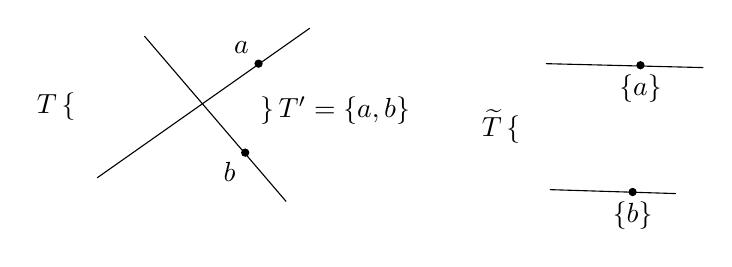
\begin{tikzpicture}[x=1cm,y=1cm]
\draw (0,0)--(2.7,1.9);
\draw (.6,1.8)--(2.4,-.3);
\fill (2.05,1.45) circle (1.5pt) node[above left] {$a$};
\fill (1.88,.32) circle (1.5pt) node[below left] {$b$};
\node at (-.5,.9) {$T\left\{\vphantom{\begin{matrix}a\\a\\a\\a\\a\end{matrix}}\right.$};
\node at (3,.85) {$\left.\vphantom{\begin{matrix}a\\a\\a\end{matrix}}\right\}T'=\{a,b\}$};
\draw (5.7,1.45)--(7.7,1.4);
\draw (5.75,-.15)--(7.35,-.2);
\fill (6.9,1.43) circle (1.5pt) node[below] {$\{a\}$};
\fill (6.8,-.18) circle (1.5pt) node[below] {$\{b\}$};
\node at (5.15,.65) {$\widetilde T\left\{\vphantom{\begin{matrix}a\\a\\a\\a\\a\end{matrix}}\right.$};
\end{tikzpicture}}

\diagram{\begin{tikzcd}
H^1(\widetilde Y)\deleted{\unsure{a}} \arrow[dr] & & \\
H^3_Y(X) \arrow[r] & H^3_{\deleted{\unsure{!}}}(X) \arrow[r,dash] & H^3(U)
\end{tikzcd}}

\diagram{\begin{tikzcd}
H^1_!(Y) & H^1_!(X) \arrow[l] \arrow[dl] & H^1_!(U) \arrow[l] \arrow[d,equal] \\
H^1_!(\widetilde Y) & & 0\quad\text{car }T\text{ connexe}
\end{tikzcd}}

\margin{$H^0($}

\diagram{\begin{tikzcd}
H^0(\widetilde T') \arrow[r] & H^0_{\unsure{!}}(\widetilde T) \arrow[r] & H^1_!(\widetilde Y) \arrow[r,no head] & H^1(\widetilde T') \\
H^0(P^2) \arrow[r] \arrow[u] & H^0(T') \arrow[r] \arrow[u] & H^1_!(X) \arrow[r,no head] \arrow[u] & \substack{H^1(P^2)\\\Vert\\\unsure{0}} \arrow[u] \\
H^0(P^2) \arrow[r] & H^0(T) \arrow[r] \arrow[u] & H^1_!(U) \arrow[r,no head] \arrow[u] & \substack{H^1(P^2)\\\Vert\\\unsure{0}}
\end{tikzcd}}

\margin{$\left\{\begin{array}{l}T\ \uline{connexe}\\T'\ \text{disconnexe},\ \deleted{\text{et}}\\\text{contenu dans }\unsure{\text{l'ou.}}\\\deleted{\text{lieu}}\ \text{de lissité},\\\text{et tte comp. de}\\T'\ \text{contient au}\\\text{plus un}\\\text{point de}\\T'.\end{array}\right.$}

\diagram{\begin{tikzcd}[column sep=large]
& & H^0(T')/\operatorname{Im}H^0(P^2) \arrow[dl,"\text{inj?}"] & H^0(T)/\operatorname{Im}H^0(P^2) \arrow[l] \arrow[d,equal] \\
H^1_!(\widetilde Y) \arrow[r] & H^0(\widetilde T/\operatorname{Im}H^0(\widetilde T') \arrow[dr,equal] & & 0 \\
& & 0 &
\end{tikzcd}}

$\deleted{\unsure{H^1_!}}$

\hrule
\scanpage{104}
% archive foliation: 103
\deleted{\unsure{pro}}

\diagram{\(\begin{array}{c@{\qquad}ccc}
& \multicolumn{2}{c}{\overbrace{\hspace{9em}}^{\text{cas propre, ou du }H^1_!}} & \\
H^1 & \begin{array}{c}\text{poids }0\\\text{niveau }0\end{array}
& \begin{array}{c}\text{poids }1\\\text{niveau }1\end{array}
& \begin{array}{c}\text{poids }2\\\text{niveau }0\end{array}\\
& & \multicolumn{2}{c}{\underbrace{\hspace{9em}}_{\text{cas lisse}}}
\end{array}\)}

\margin{morceaux purs sont semi-simples}

\diagram{\(\begin{array}{c@{\qquad}c|ccccc}
& \multicolumn{1}{c}{} & \multicolumn{3}{c}{\overbrace{\hspace{13em}}^{\text{cas propre}}} & & \\
H^2_{\deleted{\unsure{!}}} & \text{poids} & 0 & 1 & 2 & 3 & 4\\
\cline{2-2}
& \text{niveau} & 0 & 1 & 2 & 1 & 0\\
& \multicolumn{1}{c}{} & & & \multicolumn{3}{c}{\underbrace{\hspace{13em}}_{\text{cas lisse}}}
\end{array}\)}

morceaux purs de poids $\ne2$ \unsure{st|sont} semi-simples.

\margin{$\Vert$}
Le morceau pur de poids $2$ est une extension par un motif de Tate $Q(-1)^r$.

$H^2_!$\qquad il semble qu'il puisse y avoir mélange de poids dans le mauvais ordre, à cause d'une extension d'un motif effectif de poids $0$ par un autre de poids $1$; en plus de cela, il \unsure{apparaît} une extension, peut-être non triviale, d'un motif effectif de poids $0$ \inserted{resp. $1$} par un autre.
\scanpage{105}
% archive foliation: 104
\fbox{\parbox{.95\linewidth}{\uline{Poids de la cohomologie \inserted{$l$-adique} d'une variété singulière ou/et non propre}. \inserted{(sur corps $k$ \unsure{p. f. $0$})}}}

\textcircled{A} \uline{Coefficients constants}

\textcircled{1} Soit d'abord $X$ lisse et \unsure{quasi-projective|quasi-projectif}, donc par résolution forte (que nous admettons).--- on aura
\[
X=X'-Y\qquad Y=\bigcup_iY_i
\]
$X'$ lisse et projective, $Y_i$ diviseurs lisses, \inserted{irred.} à croisements normaux mutuels. \deleted{\unsure{Si}} On a donc
\diagram{\begin{tikzcd}[column sep=small]
\inserted{H^{i-1}(X')} \arrow[r] & \substack{\inserted{H^{i-1}(Y)}\\\deleted{\unsure{R^if_!}}} \arrow[r] & H^i_!(X) \arrow[r,dash] & H^i(X') \arrow[r,dash] & H^i(Y) \arrow[r,dash] & H^{i+1}_!(X) \arrow[r] & \cdots
\end{tikzcd}}

\margin{\diagram{\begin{tikzcd}
X \arrow[r,phantom,"\subset"] \arrow[d,"f"'] & X' \arrow[dl,"f'"]\\
\operatorname{Sp}k &
\end{tikzcd}}}

\deleted{\unsure{donc}} donc les poids dans $H^i_!(X)$ [qui se déterminent via val. absolues de val. propres de Frob, par réduction au cas d'un corps de type fini \unsure{\ldots}) \unsure{sont contenus} dans ceux de $H^i(X')$ [\unsure{réduits} à $i$ par Weil] et ceux de $H^{i-1}(Y)$.

On a
\[
H^{\unsure{n}}(Y)\Longleftarrow E^{pq}_2
=H^p(i_0\ldots i_r\longmapsto H^q(Y_{i_0}\cap\cdots\cap Y_{i_r}))
\]
\inserted{on peut se borner ici aux cochaines \uline{alternées}}
\margin{$\left\{\begin{array}{l}
\text{de poids }q\\
\text{de niveau }\le q\\
[\text{intéressant si}\\
i\unsure{=|\equiv}p+q\le n-1]\\
\text{de niveau }\le\unsure{2n-i-q}\ \deleted{\unsure{q}}\\
[\text{si }i=p+q\ge n]
\end{array}\right.$}
\margin{$(2n-i)-q$}

\deleted{Donc} Or ici $Y_{i_0}\cap\cdots\cap Y_{i_r}$ est projectif et lisse (de dimension $n-r-1$ si $X$ \deleted{\unsure{est}} purement de dim $n$). Donc le poids des termes $E^{pq}_2$ est $q$, et on trouve que le poids de $H^j(Y)$ est $\le j$. Donc :

\deleted{\unsure{Proposition}} \uline{Proposition 1} $H^i_!(X)$ est de poids \inserted{entre $0$ et} $\le i$. La partie de poids $i$ (resp. de poids $\le i-1$) est le quotient image de $H^i_!(X)\mathbin{-}H^i(X')$ [resp. l'image de $H^{i-1}(Y)\longrightarrow H^i_!(X)$). De plus, si $i\ge n=\dim X$, alors le \uline{niveau} de $H^i_!(X)$ est $\le2n-i$, et les deux \unsure{derniers} morceaux précédents sont de niveaux $\le2n-i-1$; de plus, il n'y a de poids qu'entre $2(i-n)$ [car il faut écrire $q\le2(n-p-1)$ !] et $i$, i.e \unsure{un gr. pondéré} d'amplitude $2n-i$ \ldots

\margin{\fbox{\parbox{.24\linewidth}{\uline{NB} Tous les morceaux de la filtration sont ``effectifs''}}}
\margin{\fbox{\parbox{.24\linewidth}{En tous cas niveau $\le\operatorname{Inf}(i,n)$}}}

Pour ce complément, notons que le niveau de $E^{pq}_2$ est $\le$ celui de $H^q(\underbrace{Y_{i_0}\cap\cdots\cap Y_{i_p}}_{\dim n-p-1})$, donc est
\[
\le \deleted{\unsure{2n-p-q}}\,
2(\deleted{\unsure{n}}n-p-1)-q
=\deleted{\unsure{2n-(p+q)}}(2n-i-2)-p
\inserted{=2(n-1)-i-p}
\quad(i=p+q)\quad\text{donc }\le2(n-1)-i
\]
\scanpage{106}
% archive foliation: 105
Donc \deleted{\unsure{négligeant}} pour $p+q=i-1$, on trouve un poids $\le2(n-1)-i+1=2n-i-1$.

\uline{Remarque} La filtration de $H^{\unsure{*}}(Y)$ déduite de la suite spectrale \unsure{est} n'est autre que la filtration par les poids. La filtration image de $H^i_!$ est donc aussi la filtration par les poids croissants (de $0$ à $i$, le dernier avec comme \unsure{noyau}) donc est également indépendante de la \unsure{comp.} \unsure{projective} $X'$ choisie. Écrivons les termes de la filtration, en utilisant le fait que $H^{i-1}(X')$ est purement de poids $i-1$, et $\deleted{\unsure{E^{i-1,0}_2}}$ que la suite spectrale est dégénérée par des raisons de poids :

\diagram{\(\begin{array}{c|c|c|c|c|c|c}
\hline
& E^{i-1,0}_2, & E^{i-2,1}_2, & \ldots & E^{1,i-2}_2, & E^{0,i-1}_2/\operatorname{Im}H^{i-1}(X'), & \operatorname{Ker}(H^i(X')\to E^{0,i}_2)\\
\hline
\text{poids} & 0 & 1 & & i-2 & i-1 & i\\
\hline\hline
\deleted{\unsure{\text{niveau}}} & & & & & &
\end{array}\)}

\deleted{\unsure{Comme $i\ge n$}} Si $i\le n$, les niveaux sont \inserted{seulement} $\le$ poids, il n'y a pas lieu à priori d'attendre plus. L'on dresse d'autre part, pour $i\ge n$, un tableau

\diagram{\(\begin{array}{c|c|c|c|c|c|c}
& \text{degré }\unsure{\text{filtrant}}\ge n & & & & &\\
& 0\ \ldots\ 0 &
\substack{\deleted{\unsure{E^{i-1,0}_2}}\\E^{2n-i-1,2(i-n)}_2} &
E^{2n-i-2,2(i-n)+1}_2 &
\ldots &
E^{0,i-1}_2/\operatorname{Im}H^{i-1}(X') &
\operatorname{Ker}(H^i(X')\to E^{0,i}_2)\\
\hline
\text{poids} & \raisebox{-1.8ex}{\Large$\times$} & 2(i-n) & 2(i-n)+1 & \ldots & i-1 & i\\
\cline{3-7}
\text{niveau} & & 0 & 1 & \ldots & 2n-i-1 & 2n-i
\end{array}\)}

\uline{Corollaire 1} (Par dualité) $H^i(X)$ est de poids compris entre $i$ et $2n$. Le morceau \deleted{\unsure{pur}} de poids $i$ est exactement l'image de $H^i(X')$. Si $i\unsure{\ge|>}n$, les niveaux des morceaux de poids $i,i+1,\ldots,2n$ sont resp. $\le2n-i,2n-i-1,\ldots,0$. Si $i\le n$ il n'y a de morceaux \deleted{\unsure{que}} que des poids
$\deleted{i,i+1,\ldots,2n\ \unsure{2(i-n)=2n-2n}}$ \deleted{\unsure{dont}}
\inserted{$i,i+1,\ldots,2i$}
qui sont de niveaux resp. $\le i,i-1,\ldots,0$.

\margin{\fbox{\parbox{.24\linewidth}{tous les morceaux de la filtration \unsure{st} ``effectifs''}}}
\margin{\fbox{\parbox{.24\linewidth}{En tous cas niveau $\le\operatorname{Inf}(i,n)$}}}
\margin{\uline{NB} les niveaux ici \uline{décroissent}}
\scanpage{107}
% archive foliation: 106
\textcircled{2} \uline{Cas \deleted{\unsure{non}} lisse non quasi-projectif.}

Si $X$ est séparé, utilisant une compactification de Nagata, et résolution des singularités \inserted{comme dessus}, on a les \unsure{ms} résultats que ci-dessus, en notant que la résolution des singularités permet de déduire les conj. de Weil pour des var. propres et lisses du cas projectif et lisse.

Si $X$ non séparé, $H^i_!(X)$ n'est plus défini. Par contre $H^i(X)$ est défini. On a, avec un \unsure{recouvrt} affine
\[
H^{\unsure{*}}(X)\Longleftarrow E^{pq}_2=H^p(\sigma\longleftarrow H^q(U_\sigma))
\]
Ici $E^{pq}_2$ est effectif de poids $\unsure{\ge|\not\ge}q$, mais \deleted{\unsure{malgré}} \deleted{\unsure{faible degré}} on peut en conclure que l'effectivité de $H^i(X)$, et le fait que ses poids sont compris entre $0$ et $2n$ si $i\ge n$, et entre $0$ et $2i$ si $i\le n$; en tous cas, ces poids sont $\le2i$, \deleted{\unsure{enfin le ni}} Enfin, on trouve que le niveau est $\le i$ \deleted{\unsure{en tous cas}, \unsure{et $\le2n-i$} (il y a de \unsure{singuliers} pour $i>n$)}.

\margin{\fbox{\parbox{.26\linewidth}{\uline{Question} le niveau ne serait-il $\le2n-i$ ? \deleted{\unsure{pour $i\ge n$}}}}}
\margin{$n=\dim X$}

\textcircled{3} \uline{Cas non lisse} : $H^i_!(X)$, ($X$ séparé). Je dis qu'il est encore vrai qu'il est \uline{effectif} et de poids $\le i$, de niveau $\operatorname{Inf}(i,2n-i)$.
Soit $U$ un ouvert lisse dense, $Y$ son complémentaire.
Donc
\diagram{\begin{tikzcd}
{} \arrow[r] & H^i_!(U)\deleted{\unsure{f}} \arrow[r] & H^i_!(X) \arrow[r] & H^i_!(Y) \arrow[r] & {}
\end{tikzcd}}
et $H^i_!(U)$ \deleted{\unsure{est}} est effectif de poids $\le i$ \inserted{de niveau $\le i$}, et $H^i_!(Y)$ aussi par hypothèse de récurrence sur la dimension, donc $H^i_!(X)$ est effectif de poids $\le i$, de niveau $\le i$. De \(=\) $H^i_!(U)$ est de niveau $\le2n-i$, et $H^i_!(Y)$ de niveau $\le2(n-1)-i\le2n-i$, on \unsure{gagne}.

\textcircled{4} \uline{Cas non lisse} : $H^i(X)$ \deleted{($X$ \unsure{séparé})}. Je dis qu'il est effectif, à poids $\uuline{\le2i}$, à niveau \deleted{$\unsure{\le\operatorname{Inf}(i,2n-i)}$ et $n=\dim X$} \inserted{$\le i$ et $\le n$}.
\inserted{Par la suite spectrale de Leray, on est ramené au cas où $X$ affine.}
Récurrence sur $i$; trivial si $i\le0$. On utilise résolution $X'\to X$, et suite spectrale de descente
\[
H^{\unsure{*}}(X)\Longleftarrow E^{pq}_2=H^p(\unsure{s|\sigma}\longmapsto H^q(\unsure{(X'/X)^s})),
\]
\deleted{\unsure{en}} \deleted{\unsure{donc}} Par hyp. de récurrence, \deleted{\unsure{pour}} \inserted{si $q<i$,} $E^{pq}_2$ est effectif

\margin{poids $\le2\operatorname{Inf}(i,n)$\\niveau $\le\operatorname{Inf}(i,n)$}
\scanpage{108}
% archive foliation: 107
de \deleted{niveau} poids $\le2q$, de niveau $\le q$. Donc il en est de même de $E^{\unsure{rs|pq}}_2$ si $p+q=i$, $p\ne0$, \inserted{et on trouve des \deleted{\unsure{poids}} poids $\le2(i-1)<2i$, des niveaux $\le i-1<i$}. Reste à examiner le terme $E^{0,i}_2\subset H^i(X')$; comme $X'$ est lisse, il est donc effectif, de poids $\le2i$, de niveau $\le i$. On a gagné ! Si on note que si $i>n$, on a $H^i(X)=0$ ($X$ affine !).

\deleted{\unsure{À priori}, $H^i(X)$ est de niveau $\le n=\dim X$. \unsure{Le tout} \illegible{4} $E^{pq}_2$ \unsure{est effectif}. \unsure{filtration} \illegible{2} \unsure{niveau}.}

\textcircled{B} \uline{Coefficients constants tordus sur $X$ lisse}, \inserted{séparé} $F$ \inserted{effectif} de poids et niveau $j$.

\textcircled{1} On suppose que les coefficients envisagés proviennent d'un motif lisse sur $X$, et \inserted{par dévissage (possible ici ?)} \unsure{on ne regarde le} cas où ce dernier est un facteur direct d'un $R^jf_*(Q_{l Y})$, avec $f:\deleted{\unsure{Z}}\mathbin{-}X$ morphisme projectif et lisse. \inserted{On peut si on veut supposer $f$ de dim relative $j$.} On est donc \unsure{ramené} au cas où
\[
F=R^jf_*(Q_{l Y}).
\]
Considérons la suite spectrale
\[
H^{\unsure{*}}(Y)\deleted{\unsure{a}}\Longleftarrow
\inserted{E^{pq}_2=}
H^p(X,R^qf_*(Y))
\]
\margin{$\unsure{p}$}

\uuline{D'après Deligne}, cette suite spectrale dégénère. Donc $H^i(X,R^jf_*(Q_l(Y)))$ \inserted{et par suite $H^i(X,F)$} apparait comme un \uline{morceau} de $H^{i+j}(Y)$. On trouve que l'on a un \deleted{\unsure{module}} \uline{effectif}, de poids \deleted{\unsure{\ne}} compris entre
$\deleted{2(n-j)\text{ et }2(i+j)}$
\uline{$i+j$} et $2(n+j)=\uline{2n+2j}$ (où $n=\dim X$);
les niveaux sont resp. $\le(2n-i+j),\ldots,0$.
Si $i\le n$, il n'y a de poids que \unsure{ceux énumérés} $i+j,i+j+1,\ldots,(2(i+j))$, de \deleted{poids} \inserted{niveaux} respectifs
$\deleted{0,\ldots,i+j}$ \inserted{$i+j,i+j-1,\ldots,0$}.

\margin{\fbox{\parbox{.27\linewidth}{peut-on remplacer $2n+2j$ par $2n+j$ ?}}}
\margin{\fbox{\parbox{.27\linewidth}{peut-on remplacer $2i+2j$ par $2i+j$ ? \deleted{\unsure{Cela fait à croire}}}}}

Résultats duaux pour $H^i_!(F)$, il est effectif à poids $\le i+j$, et \deleted{à niveaux} si $i\ge n$, il est à niveaux croiss. de $0$ à $\deleted{2n-i+j}2(n+j)-(i+j)=2n-i+j$, pour des poids croissants \unsure{ds}.

\margin{\fbox{\parbox{.27\linewidth}{les poids sont-ils $\ge j$}} \deleted{\unsure{donc}}}

Si $X$ est \uline{propre}, on trouve que $H^i(X,F)$ est pur de poids $i+j$ (et semi-simple ici\ldots)!
\scanpage{109}
% archive foliation: 108
\textcircled{2} Cas où on dispose seulement d'une représentation de $F$ sous forme sympathique \uline{localement} sur $X$ pour la top (Zar). Dans ce cas,
\deleted{on ne peut plus utiliser \unsure{comme} \unsure{puisque} $X$ séparé, \unsure{on doit en faire en localisant} sur $X$ \unsure{un sens} (\unsure{ét}), et utiliser la suite spectrale de Leray d'un recouvrement. On trouve \unsure{un énon. d'effectivité}, poids entre $0$ et $2n+2j$}
on a intérêt à travailler \uline{d'abord} avec la cohomologie à support propre sur $X$, qui permet de découper $X$ en morceaux, et d'obtenir les $=$ résultats que dessus. On déduit l'analogue en cohomologie à supports quelconques par dualité.

\deleted{Si $F$ est sympathique}

\uline{Remarque} [En fait, on voit par ce raisonnement que, en ce qui concerne la coh. à support propre, les résultats sont obtenus en supposant seulement que $F$ soit ``joli par morceaux'' sur $X$; \inserted{la lissité de $X$ par Poincaré}. Le fait $F$ \unsure{const.|const. et} tordu \inserted{sur $X$ lisse} est alors utilisé \deleted{\unsure{dans le cas lisse}} pour pouvoir procéder par dualité.

\textcircled{C} \uline{Cas de coefficients effectifs de (poids $j$, niveau $j$)} $j$ \uline{\unsure{quelc.}};
$X$ quelconque.

1) Cas de la cohomologie $H^i_!$ : déjà traité dans la remarque précédente : résultat le $=$ que dans \textcircled{B}.1).

2) Cas de la cohomologie $H^i(X,F)$. Je dis qu'il est \uline{effectif}, de poids \deleted{\unsure{entre $0$ et $2i$}} \inserted{$\le\operatorname{Inf}(2i,2n)=2\operatorname{Inf}(i,n)$}, de niveau $\le\operatorname{Inf}(\unsure{2i|i},n)$, où $n=\dim X$. \deleted{\unsure{Cas propre pour}} \ldots

\margin{?}
\scanpage{111}
% archive foliation: 110

Faisceaux $l$-adiques admissibles et motifs virtuels.

\deleted{1. Soit $S$ un schéma; $F$ un $\mathbb Q_l$}

1. On se fixe un nb premier $l$. Les schémas envisagés sont premiers à $l$. (\uline{le cas le plus intéressant est celui des schémas loc. de type fini sur $\mathbb Z$}.) Les faisceaux envisagés sont les $\mathbb Q_l$-faisceaux \inserted{constructibles}. On note $\mathbb Q_l(1)$ le faisceau de Tate $T_l(G_m)\otimes_{\mathbb Z_l}\mathbb Q_l$, et le twist par sa puissance tensorielle $n$-ième est noté $F\longmapsto F(n)$.

\margin{se borner pour commencer à ce cas!}

\margin{On travaille ds la catégorie des faisceaux $l$-adiques \unsure{constants tordus} \illegible{1}.}

2.1 Un faisceau $F$ sur $S$ est dit \uline{spécial} \inserted{\uline{de poids $i$}} (s'il est isomorphe à un \deleted{facteur direct} \inserted{\unsure{quotient constant tordu}} d'un \inserted{sous} faisceau \inserted{constant tordu d'un faisceau} de la forme $R^i f_*(\mathbb Q_{lX})$, où $f:X\longrightarrow S$ est projectif et lisse \inserted{de dim relative $i$ \unsure{ptt}}). On note que si $i<0$, cela implique $F=0$; si $i=0$, alors \deleted{\unsure{ce qui}} \deleted{\unsure{implique}} \inserted{équivaut à:} $F$ localement constant.$^{(*)}$

\margin{Définition \unsure{canulée|annulée}: dire qu'on se ramène à cette situation de \unsure{t.f.} sur $\unsure{\operatorname{Sp}|\operatorname{Spec}}\mathbb Z$.}

\margin{$(*)$ \deleted{\unsure{effectif}, \illegible{3} \unsure{étale} \illegible{2} poids $i$, \illegible{2} quotient \illegible{3} \unsure{non} \illegible{3} $\mathbb Q_l$ \illegible{2} \uline{\unsure{admissible}}!}}

\uline{Lemme} 2.\unsure{2|1}.

a) Stabilité de ``spécial de poids $i$'' \inserted{\unsure{sous-objets} et quotients cst tordus, et} par sommes directes.

b) Si $F,\unsure{F'}$ sont spéciaux de poids respectifs $i,j$, alors $F\otimes \unsure{F'}$ est spécial de $i+j$.

c) Stabilité par image inverse.

d) Si $F$ spécial de poids $i$, $\check F(-i)$ l'est aussi.

e) $\mathbb Q_l(-i)$ est spécial de poids $2i$ pour $i\geq 0$,

a) Se prouve en introduisant un $\coprod_{1\leq i\leq n}X_i$.

b) Se prouve en considérant un $X_1\times_S X_2$, et utilisant Künneth.

c) Par th. de changement de base.

d) \uline{Par th. de Lefschetz} en cohomologie $l$-adique.

\margin{d) on admet Lefschetz}

e) On \deleted{\unsure{prend}} a $\mathbb Q_l(-i)=R^{2i}f_*(\mathbb Q_{l\mathbb P^i_S})$.

\margin{\uline{Cor} 2.\unsure{3|2} Si $F$ spécial de poids $i$, et $n\geq i$, alors $\check F(-n)$ est spécial de poids $2n-i$}

3.1 Un faisceau $F$ sur $S$ est dit \uline{effectivement admissible} si \inserted{pour tout ouvert affine $U$ de $S$} l'on peut en trouver une \deleted{filtration \unsure{dont les quotients}} \inserted{filtration de $F|U$ dont les quotients} successifs sont de la forme $i_!(G)$, où $i:Y\longrightarrow \deleted{X}\inserted{U}$ est une immers. de présentation finie et $G$ sur \deleted{$\unsure{S}$} $Y$ est \deleted{\unsure{sont de la forme} \unsure{image directe} \unsure{des} \unsure{ouverts de} $U$ \unsure{des parties}} \deleted{\unsure{des faisceaux} \unsure{admissibles} \unsure{les} $F|S_{\unsure{\alpha}}$ \unsure{sont}} -admissible.

\margin{Il faut se permettre une extension \unsure{finie surj. loc.} \unsure{radicielle} de $Y$, pour rendre $G$ spécial}

\deleted{On dit} Si $\Phi$ est une partie de $\mathbb Z$, on dit que $F$ est à poids $\subset\Phi$ si \deleted{les $F|S_{\unsure{\alpha}}$ sont} \inserted{on peut prendre les $G$} admissibles de poids $\in\Phi$. (\uline{De eff admissible} alors $F$ est de poids $\subset\Phi'$, pour tt $\Phi'\supset\Phi$). Si \deleted{$\unsure{\Phi\subset E}$ est} \deleted{$\Phi$, cela implique} $\Phi$ ne contient pas d'entiers $\geq0$, cela implique $F=0$.

\margin{Attention, il n'est pas tautologique que si $F$ est eff! adm. à poids $\in\Phi$ et à poids $\subset\Phi'$, \uline{il soit} à \deleted{poids} \inserted{poids} $\subset\Phi\cap\Phi'$, \unsure{même} $\Phi\cap\Phi'=\varnothing$.}
\scanpage{112}
% archive foliation: 111

\deleted{d) Si $F$ spécial de \unsure{poids}}

\uline{Proposition} \unsure{3.3}.

a) Stabilité de ``eff. adm. de poids $\subset\Phi$'' par sous-faisceaux constructibles, quotients constructibles, \inserted{sommes finies,} extensions.

b) Si $F,F'$ sont eff adm à poids $\subset\Phi,\Phi'$, alors $F\otimes F'$ est admissible à poids $\subset\Phi+\Phi'=\{i+i'\mid i\in\Phi,\ i'\in\Phi'\}$.

c) Stabilité par \unsure{chgt} de base

d) Si $F$ est \deleted{spécial}\inserted{eff$^{\unsure{t|!}}$} admissible \uline{constant tordu} à poids $\subset\Phi$, \unsure{et} si $i\in\Phi\Rightarrow i\leq n$, alors $\check F(\unsure{-n})$ est \inserted{eff$^{\unsure{t|!}}$} admissible (constant tordu) à poids $\subset2n-\Phi=\{n-i\mid i\in\Phi\}$.

\margin{d) on admet Lefschetz}

\uline{Dém} a) b) c) sont immédiats, en utilisant les assertions correspondantes de 2.1. Notons d'ailleurs:

3.2. \inserted{Supposons $S$ qu. cpt qu. sép.} Pour que $F$ soit eff$^{\unsure{t|!}}$ adm. à poids $\subset\Phi$, il f et s. que l'on puisse trouver une partition de $S$ en \deleted{\unsure{finaux}} sous-schémas $S_i\xrightarrow{\alpha_i}S$, $\alpha_i$ immers. de prés. finie, avec \deleted{\unsure{des}} $F|S_i=F_i$ admettant une filtration dont les quotients successifs sont spéciaux de poids $\in\Phi$.

\margin{\figure{\begin{tikzpicture}[x=1cm,y=1cm]
\draw[->] (0,0) .. controls (-.7,.05) and (-.4,1.7) .. (-.4,2.1) .. controls (-.5,3.8) and (-1.3,5.2) .. (-.55,6.7);
\end{tikzpicture}}}

Comme, pour $F$ constant tordu, la formation de $\check F$ commute au changement de base, \inserted{3.\unsure{3|2}} d) résulte de 2.2.

\deleted{\unsure{ptt}}

4.1 Un faisceau $F$ est dit eff$^{t}$-admissible de niveaux $\leq\unsure{\nu|\gamma}$ si \deleted{il est effectivement admissible, et} dans 3.1, on peut prendre $G$ \deleted{de poids $j\in\unsure{\Phi}$} de la forme $G'(-k)$, $k\geq0$, où $G'$ est spécial de poids \deleted{$\unsure{j\in\Phi}$} $\leq\unsure{\nu|\gamma}$. --- On dit que $F$ est eff$^{t}$ admissible ``de poids $\subset\Phi$, et de niveaux $\leq\nu$'' si on peut choisir dans 3.1. $G'$ \deleted{\unsure{de}} spécial de poids $j\leq\nu$, avec \deleted{poids} $j+2k\in\Phi$.

\margin{\unsure{bloquer après 3.2, en énoncé analogue: 3.2 pour soit 3.1 ou} \deleted{\unsure{donc}} \unsure{que} 4.1.}

\uline{Attention}, à priori cela est plus fort que la \uline{conjonction} de ``de poids $\subset\Phi$'' et ``de niveaux $\leq\nu$''. \deleted{\unsure{Pour cela} \illegible{2} \unsure{poids}, \unsure{on a}} \inserted{On notera que si} \deleted{$\unsure{\Phi\leq d}$} $\nu$ est \deleted{\unsure{un entier}} un entier tel que $\Phi\leq\nu$ (i.e $j\in\Phi\Rightarrow j\leq\nu$), \deleted{$\unsure{\frac{n}{2}}$ \unsure{est} $\unsure{j\in\Phi}$} alors ``eff$^{\unsure{t|!}}$ adm. de poids $\in\Phi$'' $\Rightarrow$ ``id et à niveaux $\leq\nu$''.
\scanpage{113}
% archive foliation: 112

\uline{Proposition} 4.2 \deleted{\unsure{a}}

a) Stabilité de ``eff$^{t}$ adm. de poids $\subset\Phi$ et niveaux $\leq\nu$'' par sous-faisceaux constr., quotients constructibles, sommes finies, extensions.

b) $F_i$ ``eff adm de poids $\subset\Phi_i$, niveaux $\leq\nu_i$'' pour $i=1,2$ implique $F_1\otimes F_2$ ``eff$^{t}$ adm. de poids $\subset\Phi_1+\Phi_2$, niveaux $\leq\nu_1+\nu_2$''.

c) Stabilité par changement de base.

d) Si $F$ \inserted{eff$^{t}$} admissible \uline{constant tordu} ``à poids \deleted{$\unsure{j}$}\inserted{$\nu+2k$} et niveaux $\leq\nu$'' (où $k\geq0,\nu\geq0$) \deleted{\unsure{et si}} alors pour tout $n\geq\nu+k$ \inserted{(soit $n=\nu+k+h$, $h\geq0$)}, $\check F(-n)$ est eff$^{t}$ admissible constant tordu, ``à poids $2n-\nu-2k=\nu+2h$, niveaux $\leq\nu$''.

\uline{Remarque}: introduire plutôt: ``à morceaux de poids $i_\alpha$, niveaux $\nu_\alpha$'', $\alpha\in\cdots$.

\uline{Théorème} 5.1. Soit $f:X\longrightarrow S$ morphisme séparé de \deleted{t.f.} \inserted{prés finie}, et $F$ sur $X$ \deleted{eff$^{t}$ admissible} \inserted{\uuline{strictement spécial}} \deleted{de poids $j$ \unsure{et niveaux} \unsure{$\nu$}} \deleted{(i.e. déf. 2.1 \unsure{sans} \unsure{de poids} $\subset\Phi$ \unsure{niveaux})} (\unsure{i.e.} déf. 1 \unsure{p108} s'applique, avec $F$ \uline{facteur direct} d'un $R^j g_*(\mathbb Q_{lY})$, où $g:Y\longrightarrow X$ \deleted{\unsure{étant}} proj. lisse). Alors $R^i_!f_{\unsure{*|!}}(F)$ est \uline{eff$^{t}$ admissible} \deleted{\uline{\unsure{assez spécial}}} à \deleted{niveaux} poids $\leq\deleted{\unsure{2}}i+j$ \deleted{\unsure{effectif}} \inserted{et niveaux $\leq\operatorname{Inf}(i+j,2n-i+j)$}.

\deleted{\unsure{poids} $\unsure{i+j}$, \unsure{niveau} $\unsure{X}$ \unsure{pour} \unsure{tout} $\unsure{i\geq n}$,}
\deleted{Si \unsure{niveau} $n=\operatorname{Sup}_{\unsure{s\in S}}\dim X_s$ et si $i\geq n$ alors les poids}
Si $n=\operatorname{Sup}_{s\in S}\dim X_s$, \deleted{$\unsure{s\in S}$} et si $i\geq n$, les poids \deleted{\unsure{et}} et niveaux \deleted{\unsure{sont}} possibles sont
\diagram{
\begin{array}{r|c|c|c|c|}
\text{poids}&2(i-n)&2(i-n)+1&\cdots&(i+j)\\ \hline
\text{niveaux}&\leq0&\leq1&\cdots&\leq2n-i+j
\end{array}
}

\margin{\uline{Utilise Lefschetz \unsure{N.} Deligne}}
\margin{$+$ résolution des singularités \inserted{forte} pour les clôtures parfaites des corps résiduels de $S$.}
\margin{$+$ $\unsure{\frac12}$ simplicité arithmétique?}

\uline{Démonstration}. On \deleted{\unsure{en}} peut supposer $F=R^j g_*(\mathbb Q_{lY})$, $g:Y\longrightarrow X$ proj. lisse. \deleted{$\unsure{F=\mathbb Q_{lX}}$}. Utilisant le th. de changement de base propre, \deleted{\unsure{on peut}} et dévissage via suite exacte de cohomologie à supports propres, on est ramené au cas où \deleted{$\exists\,S'\longrightarrow S$} $S$ est affine, \unsure{exclt}, intègre, \inserted{$X$ affine,} $\exists\,S'\longrightarrow S$ morphisme fini plat radiciel, tel que $X' = X\times_S S'$ est \uline{lisse} sur $S'$, et se ``compactifie'' en un $\widehat X_{S'}$ \deleted{tel que $X'$} projectif et lisse, tel que $\widehat X_{S'}-X_{S'}$ soit un diviseur à croisements normaux relatifs, à composantes irréductibles \uline{lisses} sur $S'$; \inserted{enfin $F$ \deleted{\unsure{sur le même}} étant \uline{spécial} de poids $j$.} Quitte à changer de notations, on peut supposer $S=S'$, et dire $X\subset X'=\widehat X$. On termine alors \inserted{si $F=\mathbb Q_{lX}$,} comme dans les notes préliminaires (partie A, 1)). [\uline{NB} On n'utilise pas la dégénérescence de la suite spectrale qui y intervient.]

\margin{à expliciter \unsure{en faisant constamment servir le principe de} 3.3 a) et 4.2 a)}
\scanpage{114}
% archive foliation: 113

\deleted{B) Cas général. On se réduit au}

Si $F$ est quelconque, on écrit que $F$ est un sous-\deleted{objet \inserted{\deleted{cst tordu}} d'un quotient \inserted{\deleted{cst tordu}} d'un $R^d f_*(\mathbb Q_{lY})$}, où $f:Y\longrightarrow X$ morphisme projectif. [Utilisant Lefschetz \deleted{et 2.1 d) \unsure{$f,g'$} \unsure{$j\geq$ dim relative}} \deleted{faible, on peut supposer que les fibres de $f$} \inserted{fort} si $j<d=\dim$ relative de $Y/X$, et remplaçant \deleted{sont de dim $j$}. $Y$ par $Y\times_X\mathbb P_X^{j-d}$ si $j>d$, on peut supposer $j=d$]

\margin{\deleted{\unsure{et} Lefschetz fort}}
\margin{voir si cette réduction est vraiment utile \ldots}

La suite spectrale
\[
R^\alpha_!(fg)(\mathbb Q_l)\Longleftarrow E^{pq}_2=R^p_!f((R^q_!g(\mathbb Q_{lX})))
\]
dégénère, \uline{par Deligne}, donc
\[
R^i_!f(F)=E^{ij}_2
\]
est $\simeq$ quotient \inserted{cst tordu} d'un ss faisceau ct tordu d'un $R^{i+j}_!\unsure{g|fg}(\mathbb Q_{lY})$.

\margin{\uuline{utilise Lefschetz fort}}
\margin{[N.B. Voir si Deligne ne peut se remplacer par \uline{\unsure{factorisation} de Artin} sur $X\longrightarrow S$, \unsure{puis} ramener au cas de $n=1$\ldots]}
\margin{semi-simplicité utilisée!}

La conclusion en résulte, en utilisant le cas précédent pour $Y\longrightarrow S$, de dim relative $\leq n+j$ \ldots

\uline{Corollaire} \unsure{5.2|5.1}. Si la partie ``\uuline{semi-simplicité}'' des conjectures de Tate est vérifiée, la conclusion de 5.1. est vraie dès que l'on suppose seulement que $F$ est eff$^{t}$ admissible de poids $j$. Par suite, si on suppose $F$ eff$^{t}$ admissible de poids $\leq\deleted{\unsure{k}}\inserted{j}$, on a un énoncé correspondant, \deleted{De} $R^i\unsure{f_*|f_!}(F)$ est \inserted{eff. admissible,} de poids $\leq\deleted{\unsure{\operatorname{Inf}}}i+j$, \deleted{\unsure{de niveau} $\unsure{i+j}$} \inserted{niveaux $\leq\operatorname{Inf}(i+j,2n-i+j)$}. Si $i\geq n$, on trouve des poids entre $2(i-n)$ et $(i+j)$, correspondant aux niveaux $0,1,\ldots,2n-i+j$.

On se ramène en effet \inserted{par dévissage et déf;} au cas où $F$ est \uline{spécial} de poids $j$, et par th. de chgt. de base propre au cas où $S$ de type fini sur $\unsure{\operatorname{Sp}|\operatorname{Spec}}\mathbb Z$, et

\margin{alors par semi-simplicité $F$ est \unsure{stt} spécial}

\uline{Cor.} 5.3 (sans conj. type Tate) \deleted{\unsure{on a}} Si $F$ est eff. admissible, Alors $R^i_!f(F)$ est eff$^{t}$ admissible.
\scanpage{115}
% archive foliation: 114

\uline{Cor.} 5.4. Sur un corps $k$, si $X$ est lisse, séparé, de t.f., et si $F$ est \deleted{\unsure{un}} str$^{t}$ spécial de poids $j$ (resp. eff$^{t}$ adm. de poids $j$, si l'on admet conjecture de $\frac12$ simplicité), alors $R^if_*(F)$ est de eff$^{t}$ admissible de poids entre $i+j$ et $2n+2j$, et les niveaux correspondants étant resp. $\leq2(n-i+j),2(n-i+j)-1,\ldots,0$. Si on a $i\leq n$, on a \deleted{les niveaux}\inserted{seulement} des poids \deleted{\unsure{et la suite de}} $i+j,i+j+1,\ldots,2(i+j)$, \deleted{\unsure{de}} niveaux correspondants étant $\leq i+j,i+j-1,\ldots,0$.

\margin{résolution, Lefschetz fort, et le cas échéant semi-simplicité}

On peut, soit procéder par dualité à partir de 5.1 et 5.2, soit reprendre \inserted{dans le cas $F$ quelc.} la dém. de 5.1 resp. 5.2, en utilisant la \deleted{suite exacte de cohomologie relative} \inserted{\unsure{trivialité|transitivité} de la suite spectrale de Leray}, pour se ramener au cas où $F$ est $\mathbb Q_l$. Dans ce cas, on peut procéder par \inserted{compactification et} résolution des singularités, pour écrire $X=\widehat X-D$, $\widehat X$ \deleted{projectif et lisse} propre et lisse et $D$ \inserted{div} à croisements normaux, et en écrivant suite exacte de ch. relative (supports quelc.) pour $X,\widehat X$ et $D$, et la suite spectrale de localisation pour $H^{\unsure{\alpha|*}}_D(\widehat X)$.

\margin{le faire à titre de vérification de cohérence du yoga!}

6. Soit $f:X\longrightarrow S$ un morphisme de t.f., et $F$ un faisceau \deleted{très spécial}\inserted{effectivement admissible} sur $X$, de poids $j$. On veut des renseignements sur \inserted{les} $R^\nu f_*(F)$, en particulier on veut qu'ils soient effectivement admissibles, de poids que nous préciserons. \deleted{Comme} \inserted{Supposons d'abord $F=\mathbb Q_{lX}$} pour le th. de finitude, on regarde d'abord le cas d'une immersion
\scanpage{116}
% archive foliation: 115

\[
X\unsure{\subset|\leftarrow}Y
\]
\[
X_0\ X_1\ \cdots
\]
\deleted{$X\unsure{\subset|\leftarrow}Y$}
\[
\mathbb Q_l
\]

\diagram{\begin{tikzcd}
X_0 \arrow[r,hook,no head,"i"'] & X \arrow[r,hook,no head,"f"'] & Y
\end{tikzcd}}
$X$ \uline{régulier}

\diagram{\begin{tikzcd}
i_!(\mathbb Q_{lX_0}) \arrow[r] & \unsure{\widehat R|R^\uparrow}i_*(\mathbb Q_{lX_0})
\end{tikzcd}}

\margin{\figure{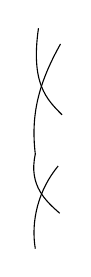
\begin{tikzpicture}[x=1cm,y=1cm]
\draw (0,2.8) .. controls (-.1,2.1) and (.1,1.9) .. (.3,1.7);
\draw (.28,2.6) .. controls (0,2.1) and (-.1,1.7) .. (-.04,1.2);
\draw (-.04,1.2) .. controls (-.13,.8) and (.1,.6) .. (.27,.45);
\draw (.25,1.05) .. controls (0,.75) and (-.1,.35) .. (-.04,0);
\end{tikzpicture}}}

\unsure{6|4}

\textcircled{1} $X$ \uline{régulier}, $\unsure{P|F}=\mathbb Q_{lX}$, $f$ immersion $(n=\dim\overline{f(X)})$.

On peut supposer $X\longrightarrow Y$ imm. \uline{ouverte}
\diagram{\begin{tikzcd}
&Y'\arrow[d,"h"]\\
X\arrow[ur,hook,no head,"g"]\arrow[r,hook,no head,"f"']&Y
\end{tikzcd}}
$Y'$ régulier, $Y'-g(X)=\deleted{\unsure{D}}h^{-1}(Y-X)=Z$ diviseur à croisements normaux $Z=\sum Z_i$.

\[
\deleted{\unsure{R}}R^*f_*(\mathbb Q_{lX})\Longleftarrow E^{pq}_2
=R^ph_*((R^qg_*(\mathbb Q_l)\unsure{(-1)|(-j)}))
\]
\[
R^qg_*(\mathbb Q_l)=\bigwedge^q\sum\mathbb Q_{lZ_i}
=\sum_{i_1<\cdots<i_q}\mathbb Q_{l\,Z_{i_1}\cap\cdots\cap Z_{i_q}}(-q)
\]
pur de poids $2q$

\margin{$X\subset$}

$E^{p0}_2=R^ph_*(\mathbb Q_{l\unsure{X'|Y'}})$ est eff$^{t}$ admissible de poids $\leq p=i$ niveaux $\leq\operatorname{Inf}(p,2n-2-\unsure{p}$

[\deleted{$\unsure{\leq2p}$} au complet si $p\geq n-1$]

\[
E^{pq}_2=\sum_{i_1<\cdots<i_q}R^pf_{Z_{i_1}\cap\cdots\cap Z_{i_q}*}(\mathbb Q_l)(-q)
\]
est eff. admissible de poids $\leq p+2q=i+q\deleted{\unsure{\leq}}\leq2n\deleted{\unsure{a}}$
de niveaux $\leq\operatorname{Inf}(p,2n-2q-p)$

\margin{$p\unsure{\leq}2(n\deleted{\unsure{a}}-q)\,/\,p$}
\margin{\textcircled{\unsure{V. l.|F. l.}} $i+q=$
$\boxed{\begin{gathered}p+2q\leq2n\deleted{\unsure{a}}\\q\leq n,2n-i\end{gathered}}$}

en tous cas, poids reste $\leq\deleted{\unsure{2}}\operatorname{Inf}(2i,2n-2$

niveaux \deleted{$\unsure{\leq i\rightarrow}$}
$\leq\operatorname{Inf}(i,2n-2-i)$

\margin{$p\leq n-1$\\$q\leq n$}

\[
\begin{array}{cc}p&\unsure{n+q|n-q}\\
\multicolumn{2}{c}{p+q\geq n}\end{array}
\]
\[
2(p-n+q)=2(i-n)\qquad 2n-2-
\]
\[
2(n-q)-p=\uline{2n-i}-q
\]

\figure{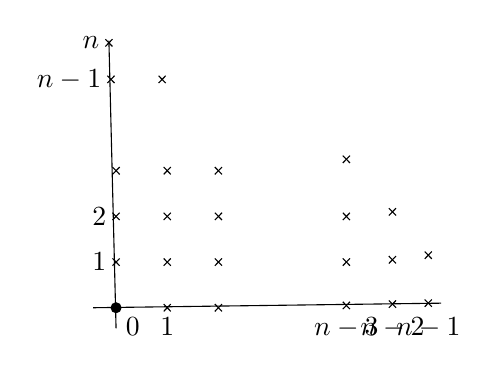
\begin{tikzpicture}[x=.65cm,y=.58cm]
\draw (-.45,0)--(6.35,.10);
\draw (0,-.45)--(-.14,5.85);
\fill (0,0) circle (2pt);
\foreach \x/\y in {0/1,0/2,0/3,-.10/5,-.14/5.8,1/0,1/1,1/2,1/3,.9/5,2/0,2/1,2/2,2/3,4.5/.05,4.5/1,4.5/2,4.5/3.25,5.4/.08,5.4/1.05,5.4/2.1,6.1/.10,6.1/1.15}
{\draw (\x-.07,\y-.08)--(\x+.07,\y+.08);
\draw (\x-.07,\y+.08)--(\x+.07,\y-.08);}
\node[below right] at (0,0) {$0$};
\node[below] at (1,0) {$1$};
\node[below] at (4.5,0) {$n-3$};
\node[below] at (5.4,0) {$n-2$};
\node[below] at (6.1,0) {$n-1$};
\node[left] at (0,1) {$1$};
\node[left] at (0,2) {$2$};
\node[left] at (-.1,5) {$n-1$};
\node[left] at (-.14,5.8) {$n$};
\end{tikzpicture}}

2.
\scanpage{118}
% archive foliation: 117

$i\leq n-1$
\diagram{\begin{array}{r|ccccc|}
\text{poids}&0&1&&&2i\\ \hline
\text{niveaux}&0&1&&&\unsure{2i|i}\\ \hline
\end{array}}

$E^{i0}_2$
\diagram{\begin{array}{r|c|c|c|c|}
\text{poids}&\unsure{0|2}&1&&i\\ \hline
\text{niveaux}\leq&0&1&&i\\ \hline
\end{array}}

$E^{i-1,1}_2$
\diagram{\begin{array}{r|c|c|c|c|c|}
\text{poids}&2&3&&i&i+1\\ \hline
\text{niveaux}&0&1&&i-2&i\unsure{-2+1|-1}\\
\end{array}}

\deleted{\unsure{donc}}
\deleted{$p+q=i$}
$E^{i-2,2}_2$
\diagram{\begin{array}{r|c|c|c|c|c|c|}
\text{poids}&4&5&\diagup\diagup&i&i+1&\deleted{\unsure{2}}i+2\\ \hline
\text{niveaux}&0&1&\diagup&i-4&i-3&i-2
\end{array}}

\margin{\deleted{$p\leq\unsure{2}(n-1-q)$}}
\margin{\deleted{$p+q\leq n-1$}}
\margin{$i$ \deleted{$\unsure{p\leq}$}}

$E^{0i}_2$
\diagram{\begin{array}{r|c|}
\text{poids}&2i\\ \hline
\text{niveaux}&0
\end{array}}

\margin{\textcircled{$i\leq n-1$}}
\diagram{\boxed{\begin{array}{r|c|c|c|c|c|c|c|c|}
\text{poids}&0&1&\cdots&i-1&i&i+1&\cdots&2i\\ \hline
\text{niveaux}&0&1&&i-1&i&i-1&&0
\end{array}}}

\margin{\textcircled{$i\geq n$}}

$E^{i0}_2$
\diagram{\begin{array}{|c|c|c|c|c|c|}
2(i-n+1)&2(i-n+1)+1&\cdots&&\deleted{\unsure{i-1}}&i\\ \hline
0&1&2&&\deleted{\unsure{i}}&2(n-1)-i
\end{array}}

$E^{i-1,1}_2$
\diagram{\begin{array}{|c|c|c|c|c|}
2(i-n)+2&2(i-n)+3&&i&i+1\\ \hline
0&1&&2n-i-2&2n-i-\unsure{1|2}
\end{array}}

$E^{i-2,2}_2$
\diagram{\begin{array}{|c|c|}
2(i-n)\deleted{\unsure{+3}}+4&2(i-n)+\unsure{3|5}\\ \hline
0&1
\end{array}\qquad
\begin{array}{|c|c|c}
i&i+1&i+2\\ \hline
2n-i-2&2n-i-3&2n-i-2
\end{array}}

$E^{i-3,3}_2$
\diagram{\begin{array}{|c|c|}
2(i-n)+6&2(i-n)+7\\ \hline
0&1
\end{array}\qquad
\begin{array}{|c|c|c|c}
i&i+1&\unsure{i+2|i+3}&i+3\\ \hline
2n-i-6&2n-i-5&2n-i-4&2n-i-3
\end{array}}

\deleted{$\unsure{E}$}
$E^{0,i}_2$
\diagram{\begin{array}{|c|}
2i\\ \hline
0
\end{array}}

\figure{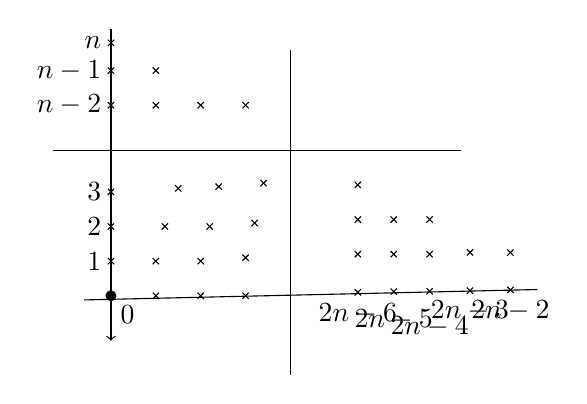
\begin{tikzpicture}[x=.57cm,y=.44cm]
\draw (-.6,-.12)--(9.5,.18);
\draw[->] (0,7.7)--(0,-1.3);
\draw (-1.3,4.2)--(7.8,4.2);
\draw (4,7.1)--(4,-2.3);
\fill (0,0) circle (2pt);
\foreach \x/\y in {0/1,0/2,0/3,0/5.5,0/6.5,0/7.3,1/0,2/0,3/0,1/1,2/1,3/1.1,1.2/2,2.2/2,3.2/2.1,1.5/3.1,2.4/3.15,3.4/3.25,1/5.5,2/5.5,3/5.5,1/6.5,5.5/.1,6.3/.12,7.1/.13,8/.15,8.9/.17,5.5/1.2,6.3/1.2,7.1/1.2,8/1.25,8.9/1.25,5.5/2.2,6.3/2.2,7.1/2.2,5.5/3.2}
{\draw (\x-.07,\y-.09)--(\x+.07,\y+.09);
\draw (\x-.07,\y+.09)--(\x+.07,\y-.09);}
\node[below right] at (0,0) {$0$};
\node[left] at (0,1) {$1$};
\node[left] at (0,2) {$2$};
\node[left] at (0,3) {$3$};
\node[left] at (0,5.5) {$n-2$};
\node[left] at (0,6.5) {$n-1$};
\node[left] at (0,7.3) {$n$};
\node[below] at (5.5,.05) {$2n-6$};
\node[below] at (6.3,-.13) {$2n-5$};
\node[below] at (7.1,-.32) {$2n-4$};
\node[below] at (8,.15) {$2n-3$};
\node[below] at (8.9,.15) {$2n-2$};
\end{tikzpicture}}

\unsure{1}

\[
q=2n-i\qquad p=2(i-n)
\]
\[
E^{2(i-n),2n-i}_2=R^{2(i-n)}f_{\unsure{Z*|Z}}(\mathbb Q_l
\]
\[
2(i-n)+2(2n-i)=2n
\]
\scanpage{119}
\margin{20.3.68\quad 1. Korrektur}

{\Large Lecture Notes in Mathematics}

A collection of informal reports and seminars

Edited by A. Dold, Heidelberg and B. Eckmann, Zürich

41\hfill\rule{0.68\linewidth}{1pt}

{\Large Local Cohomology}

A Seminar given by A. Grothendieck

Notes by R. Hartshorne

1967\hfill\rule{0.68\linewidth}{1pt}

\figure{

\begin{tikzpicture}[x=0.65cm,y=0.65cm,line width=0.8pt]
\draw[fill=black] (0.1,3.1) .. controls (0.55,3.0) and (0.8,2.6) .. (0.73,2.0)
--(-0.2,2.0) .. controls (-0.15,2.3) and (0.0,2.4) .. (0.15,2.5)
--(-0.35,2.35)--(-0.57,2.54)--(-0.33,2.88)--(-0.17,3.02)--(-0.16,3.27)--(0.02,3.22)--cycle;
\draw[white,line width=1.5pt] (0.2,3.05) .. controls (0.49,2.88) and (0.56,2.5) .. (0.47,2.12);
\draw[fill=white] (-0.35,2.59)--(-0.14,2.91)--(0.09,2.98)
.. controls (0.34,2.75) and (0.1,2.48) ..(-0.03,2.35)--(-0.12,2.1)--(0.36,2.1)
.. controls (0.5,2.6) and (0.39,3.0) ..(0.1,3.1)--cycle;
\fill (-0.04,2.94) circle (0.045);
\draw (-0.2,1.97)--(0.63,1.97)--(0.54,1.82)--(-0.1,1.82)--cycle;
\draw (-0.05,1.82) .. controls (-0.65,1.93) and (-0.48,1.48) .. (-0.14,1.52)
--(-0.31,1.2)--(0.69,1.2)--(0.47,1.52)
.. controls (0.93,1.43) and (1.0,1.93) ..(0.54,1.82);
\draw (0.17,0) ellipse (0.99 and 1.26);
\draw (0.17,0) ellipse (0.89 and 1.17);
\fill (0.17,0) ellipse (0.55 and 0.91);
\node[text=white,font=\Huge] at (0.16,0.1) {S};
\node[text=white,font=\Large] at (0.22,-0.34) {J};
\node[rotate=76,font=\tiny] at (-0.59,-0.34) {ALLE};
\node[rotate=23,font=\tiny] at (-0.17,0.99) {ZEIT};
\node[rotate=-72,font=\tiny] at (0.98,0.12) {WACH};
\node[font=\tiny] at (0.18,-1.08) {\unsure{1842|184}};
\draw[line width=1.5pt] (-0.9,1.37) .. controls (-1.43,1.65) and (-1.6,1.05) ..(-1.22,1.12)
.. controls (-0.83,1.18) and (-0.96,0.79) ..(-1.05,0.64);
\draw[line width=1.5pt] (1.02,1.39) .. controls (1.6,1.7) and (1.75,1.02) ..(1.35,1.13)
.. controls (1.01,1.2) and (1.08,0.71) ..(1.21,0.63);
\draw (-1.41,1.01) .. controls (-1.57,0.33) and (-1.48,-0.53) ..(-1.12,-1.02);
\draw (-1.25,0.96) .. controls (-1.36,0.19) and (-1.23,-0.44) ..(-0.98,-0.8);
\draw (1.57,1.02) .. controls (1.77,0.16) and (1.47,-0.61) ..(1.27,-0.98);
\draw (1.41,0.96) .. controls (1.51,0.25) and (1.32,-0.49) ..(1.1,-0.87);
\draw (-0.87,-0.92) .. controls (-0.71,-1.13) and (-0.83,-1.36) ..(-0.54,-1.43)
.. controls (-0.23,-1.27) and (-0.16,-1.61) ..(-0.4,-1.75);
\draw (1.04,-0.94) .. controls (0.88,-1.17) and (1.04,-1.37) ..(0.7,-1.45)
.. controls (0.42,-1.28) and (0.33,-1.62) ..(0.57,-1.75);
\draw[line width=1.5pt] (-0.69,-1.65) .. controls (-0.22,-2.17) and (-0.12,-1.78) ..(0.01,-1.71);
\draw[line width=1.5pt] (0.46,-1.72) .. controls (0.72,-1.94) and (0.82,-1.84) ..(1.0,-1.59);
\draw[line width=1.3pt] (-0.37,-2.06)--(-0.07,-2.06)
.. controls (0.1,-2.28) and (0.3,-2.28) ..(0.47,-2.06)--(0.73,-2.06);
\end{tikzpicture}}
% crop-candidate: scan 119

Springer-Verlag \(\cdot\) Berlin \(\cdot\) Heidelberg \(\cdot\) New York
% archive foliation: 118
\scanpage{120}
\(\boxed{i\ge n}\)
\diagram{\[
\boxed{\begin{array}{c|c|c|c|c|c|c|c|c}
\text{poids}&2(i-n)+2&2(i-n)+3&\unsure{2(i-n+4)|2(i-n+2)}&
\deleted{i}&i+1&i+2&\cdots&2n\\ \hline
\text{niveaux}&0&1&2&\deleted{2n-i-2}&2n-i-1&2n-i-2&\text{---}&0
\end{array}}
\]}
\figure{\begin{tikzpicture}
\draw[->] (0,0)--(3.2,.7);
\draw[->] (3.8,.65)..controls (5,.55) and (6,.15)..(7,0);
\end{tikzpicture}}

poids \(2n\) s'identifie avec
\[
\deleted{\unsure{R^{2n}}}\quad
E_2^{2(i-n),2n-i}
=\sum R^{2(i-n)}f_{\underbrace{Z_{\alpha_1}\cap Z_{\alpha_2}\cap\cdots\cap Z_{\alpha_{2n-i}}}_{\dim\,i-n}}
(Q_l)(\unsure{2n-i|-2n+i})
\]
\[
2n-i\le n\le i\qquad n-(2n-i)=i-n
\]
\[
2(i-n)+2(2n-i)=2n
\]
\diagram{\[
\boxed{\begin{array}{c|c|c|c|c|c|c|c|c|c@{\qquad}c}
i&0&1&\cdots&n-1&n&n+1&\cdots&2n-1&\deleted{2n}&\le2n-1\\ \hline
\text{niveaux}&0&1&\cdots&n-1&n-1&n-2&\cdots&0&&\le n-1\\ \hline
\text{poids}\le&0&2&&2n-2&2n&2n&2n&2n&&\le2n
\end{array}}
\]}
\[
\boxed{\begin{array}{ll}
\text{poids}&\le2\operatorname{Inf}(\unsure{i},\unsure{n})\\
\text{niveaux}&\le\operatorname{Inf}(i,n-1)
\end{array}}
\]

\noindent\rule{0.75\linewidth}{.4pt}

\margin{Si \(F\), \unsure{stt!|strt!} spécial de poids \(\unsure{i|j}\)}
\[
\begin{array}{ll}
\text{poids}&\le2\operatorname{Inf}(i,n)+j\quad ?\\
\text{niveaux}&\le\operatorname{Inf}(i,n-1)+j
\end{array}
\]
\deleted{\(\boxed{2^\circ}\quad f\) \illegible{2},
\[
\unsure{F}=Q_l
\]}
Cas général

\unsure{relation conjecturée} \illegible{2}

\margin{au vois. de \(\deleted{\unsure{x}}\,y\)}
\diagram{\[
\begin{tikzcd}
X\arrow[d,"f"]\\
Y\ni y
\end{tikzcd}
\]}
\[
n=\deleted{\unsure{d_y}}\ d_y(\unsure{f|\varphi})
=\underset{\substack{x\in X\\ \text{tq }f(x)\in\unsure{\operatorname{Sp}^{0}_{Y,y}|\operatorname{Sp}_{Y,y}}}}{\operatorname{Sup}}
\left[\deg\unsure{\operatorname{tr}}[k(x):k(f(x))]
+\deleted{\unsure{d}}\dim\left(\frac{\overline{f(x)}}{\unsure{Y_y}}\right)\right.
\]
\[
\boxed{\begin{array}{ll}
\text{poids}&\le2\operatorname{Inf}(i,n)+j\\
\text{niveaux}&\le\operatorname{Inf}(i,\unsure{n})+j
\end{array}}\quad ?
\]
\margin{\unsure{peut on remplacer par} \(n-1\)
\unsure{si} \(f\) \deleted{\unsure{à fibres} \illegible{1}}
de dim \(\le n-1\) ?}
% archive foliation: 119
\scanpage{122}
2) \(F\) \deleted{\(\unsure{=Q_{lX}}\)} strictement spécial
\inserted{de poids \(j\)}, \(X\) régulier.

\diagram{\[
\begin{tikzcd}[name=diag122,execute at end picture={
\draw[rounded corners] (-.35,.95) rectangle (1.5,-.15);
}]
X'\arrow[r,hook,no head,"f'"]\arrow[d,"p"']&
Y'\arrow[d,"q"]\\
X\arrow[r,hook,"f"']&\deleted{X}\,\unsure{Y}
\end{tikzcd}
\]}
Cas très spécial
\[
F=R^{\unsure{d|j}}p_*(Q_{lX'}),
\]
\margin{\(p\) de dim relative \(j\)}

On a alors
\[
R^\alpha(fp)_*(Q_{lX'})
\Longleftarrow E_2^{pq}=R^pf_*(R^q\unsure{g_*|p_*}(Q_l))
\]
suite spectrale qui \uline{dégénère} par Deligne,
d'où
\[
\unsure{R^if_*}(F)=R^if_*(R^j\unsure{g_*|p_*}(Q_{lX'}))
\]
est un \uline{morceau} de
\[
R^{i+j}(fp)_*(Q_{lX'})
\]
Or
\[
R^\alpha(fp)_*(Q_{lX'})
\Longleftarrow \unsure{E}_2^{pq}=R^pq_*(R^qf'_*(Q_{lX'}))
\]
Or \(Y'\) est de dim \(\deleted{\unsure{n+j}}\,n'\le\boxed{n+j}\)

donc \(R^qf'_*(Q_{lX'})\) est effectif de poids
\[
\le2\operatorname{Inf}(\unsure{2q|q},\unsure{2n+2j|n+j})
\]
de niveau
\[
\le\operatorname{Inf}(q,n+j-1)
\]
\(q\) est de dim relative \(\le\)

\deleted{On prend \(p+q=i+j\)}

\deleted{\unsure{a priori}} \(E_2^{pq}\) de poids \(\le\)
% archive foliation: 121
\scanpage{125}
\uline{Dévissage de \(Q_l\)-faisceaux}

\deleted{Un faisceau}

Un \(\unsure{\mathbb Q_l|Q_l}\)-faisceau \deleted{est dit} \inserted{\(F\)} sur \(X\) est dit
\uline{admissible} \inserted{de type \(\le d\)}, s'il satisfait la condition suivante :

\(\forall x\in X\), existe voisinage ouvert \(U\) de \(x\) dans \(\overline{x}\)
et filtration \inserted{finie} de \(F|U\) par des ss-faisceaux
\deleted{\(\unsure{F^i}\)}
tels que les \(\operatorname{gr}^i(F|U)\) soient isomorphes
à un \deleted{``facteur''}
\inserted{\unsure{quotient} \unsure{ess. const.} d'un \unsure{sous-quotient|ss-quotient} \unsure{ess. const.}}
d'un faisceau de la forme
\[
R^ng_*(\deleted{\unsure{Q_{lV}}}\ Q_l),
\]
où \(g:V\mathbin{-}U\) est un morphisme \uline{projectif},
\unsure{et} \uline{lisse}, à fibres connexes \inserted{de dim \(\le d\)}.

\margin{``\unsure{ess. const.}'' signifie : faisceau à \unsure{struc.-disc.|structure discrète}}

[se vérifie fibre par fibre, \(+\ F\) est ``constructible'']

\deleted{\unsure{Cela est} \unsure{que} \(F\) \unsure{est} \illegible{1}}
\inserted{\unsure{en tous cas} \uline{par} \uline{fibre} \uline{géom}}

\uline{Lemme 1}\quad
Les \deleted{\unsure{fi}} \(\unsure{\mathbb Q_l|Q_l}\)-faisceaux admissibles de type \(\le d\)
forment une sous-catégorie abélienne
\deleted{\unsure{exacte} et épaisse (stable par}
\inserted{\uline{épaisse} de la catégorie des}
\inserted{\(Q_l\)-faisceaux constructibles}
\deleted{noyaux, conoyaux, extensions) de la catégorie des}
\deleted{\(\unsure{\mathcal F}\)}
est stable par ss-\deleted{\unsure{fais}}objets et objets quotients.

En effet, si \(F|U\) est muni d'une filtration \(d\)-spéciale,
\inserted{et si \(G|U\) est \unsure{ess. const.},}
alors la filtration induite sur \(G\) ou \((F|U)/G\) est \(d\)-spéciale,
\deleted{car \(H_d\)}
est stable par extensions : trivial.

\uline{Lemme 2}\quad \uline{Images inverses}\hfill trivial.
% archive foliation: 124
\scanpage{127}
\uline{Lemme 3}\quad
Soit \(f:X\mathbin{\text{---}}Y\) un morphisme
\inserted{compactifiable} de type fini, de dim relative \(\le d'\),
\(F\) un \(\unsure{Z_l|Q_l}\)-faisceau admissible de type \(\le d\) sur \(X\),
alors pour \deleted{\unsure{tout}} \(i\), \(R^i_!f(F)\) sur \(Y\)
sont admissibles de type \(\le d+d'\).
\figure{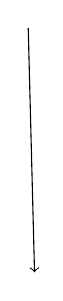
\begin{tikzpicture}\draw[->] (0,3.1)--(.08,0);\end{tikzpicture}}

On peut supposer \(Y=\operatorname{Sp}k\), \(k\) un corps.

Récurrence sur \(d+d'\), trivial si \(d'\le0\).
Supposons \(d+d'>0\), et le th. démontré pour les
\deleted{\unsure{d'}} \inserted{\(\delta'<d'\)}.

Soit \(U\subset X\) \inserted{ouvert} lisse sur \(k\) et dense dans \(X\),
et \inserted{que \(F|U\) ait une filtration \(d\)-admissible.}
[N.B. on est obligé dans la déf. plus haut d'admettre une extension radicielle sur la base.]
et soit \(Z=X-U\).

On a
\[
R^n_!f_U(F|U)\longrightarrow R^n_!f_*(F)
\mathbin{\text{---}} R^n_!f_{\unsure{Z}*}(F|\unsure{Y|Z})
\]
ce qui nous ramène au cas de \(f_Z\) et \(f_U\) grâce aux lemmes 1 et 2;
le cas de \(f_Z\) est connu par l'hyp. de réc.,
et \deleted{alors} \unsure{pour le cas où} \(X\) est lisse
sur \(k\) et a une filtration \(d\)-admissible.

Par dévissage et le lemme \(1\unsure{a|er}\) on peut supposer que \(F\)
est un quotient \inserted{\unsure{ess. const.}} d'un
% archive foliation: 126
\scanpage{129}
sous-module \inserted{\unsure{ess. const.}} d'un \(R^mg_*(\unsure{\mathbb Q_l|Q_l})\),
\(g:V\mathbin{\text{---}}U\) un morphisme \uline{projectif} de dim
\inserted{relative} \(\le d\).
On a donc des suites exactes
\[
0\longrightarrow \underset{\unsure{/}}{G}\mathbin{\text{---}}
R^mg_*(\unsure{\mathbb Q_l|Q_l})\mathbin{\text{---}}H\mathbin{\text{---}}0
\]
\[
0\mathbin{\text{---}}\underset{*}{I}\mathbin{\text{---}}
\underset{*}{G}\mathbin{\text{---}}F\longrightarrow0
\]
et \uline{de} nouvelles applications du lemme 2 nous ramènent au cas des \(I\) et \(G\),
\(R^nf_*(F)\) lorsque \deleted{\(I\subset G\)}
\(F\) \unsure{ess. const.} \(\subset R^mg_*(\unsure{\mathbb Q_l|Q_l})\).
Pour continuer, il faut utiliser le
\uline{``th.'' de complète réductibilité}
pour nous ramener au cas où \(F\) est de la forme \(R^mg_*(\unsure{\mathbb Q_l|Q_l})\)
on doit donc examiner le cas
\[
R^p_!f_*(R^qg_*(Q_l))\qquad p,q\ge0
\]

\deleted{(\unsure{N°|1°}) Cas \(m=0\). Nous procédons par réc. \uline{descendante}
sur \(p+q\) \unsure{supprimé}, en supposant que c'est vrai pour \((p',q')\)
si \(p'>p\) \uline{ou} \(q\)}
% archive foliation: 128
\scanpage{131}
De plus, procédant par récurrence sur \(d+d'\), et utilisant une
\uline{factorisation d'Artin} de \(U\)
[ce qui est loisible, car l'on peut prendre \(U\) petit],
on est ramené au cas où \(U\) est de \uline{dim 1}.

Alors la suite exacte pour \(\deleted{\unsure{g}}fg\),
\deleted{\unsure{se}}
compte tenu de
\[
R^0_!f(R^q_!\unsure{g_*|g}(Q_l))=0,
\]
se réduit à \deleted{des} suites exactes courtes
\[
\begin{array}{l}
0\mathbin{\text{---}} R^2_!f_*(R^{n-2}g_*(Q_l))
\mathbin{\text{---}}\unsure{R^n(gf)_!|R^n_!(fg)_*}(Q_l)
\mathbin{\text{---}}R^1_!f_*(R^{n-1}g_*(Q_l))\\
\hfill\mathbin{|}\\[-4pt]
\hfill0
\end{array}
\]
donc par lemme 1 on est ramené à vérifier que
\[
R^n_!\overbrace{\unsure{gf|fg}}^{h}\unsure{_{!*}|_*}(Q_l)
\]
est spécial.
On utilise la résolution des singularités pour \(V\),
on a \(V=\widehat V-Z\), \(\widehat V\) projectif et lisse sur \(k\), d'où
\[
R^{n-1}_!h_Z(Q_l)\longrightarrow
R^n_!\unsure{\widehat h|h}(Q_l\longrightarrow
R^n_!\widehat h(Q_l)
\]
% archive foliation: 130
\scanpage{133}
et \deleted{\(\unsure{F}\)} par lemme 1 il suffit de regarder les \uline{extrêmes}.
Celui de droite est O.K. \deleted{\unsure{connu}} par \uline{définition},
celui de gauche par hyp. de récurrence. O.K.

\uline{Proposition 4}\quad
Soit \(i:U\mathbin{\text{---}}X\) une immersion ouverte,
\inserted{sur \(X\) excellent, de dim \(\le d\),}
\(F\) un \deleted{\unsure{le}} \(Q_l\)-faisceau
\deleted{\(\unsure{d}\)}\inserted{\(d'\)}-admissible.
Alors les \(R^ni_*(F)\) sont
\(\unsure{(d+d'\deleted{2}\inserted{1})|(d+d'-1)}\)-admissibles.
\figure{\begin{tikzpicture}\draw (0,2)--(0,0);\end{tikzpicture}}

Récurrence sur \(d+d'\),
\deleted{En effet, soit \inserted{\unsure{de façon que}}
\(\unsure{W|V}\subset U\), \(\unsure{W|V}\) dans \(U\), tel que
\(\unsure{F\vert W|F\vert V}\) \illegible{1}.}
\inserted{trivial si \(d+d'=0\) donc \(d=0,d'=0\).
Supposons \(d+d'>0\), et \deleted{\unsure{est}} \unsure{prouvé} si
\(\delta+\delta'<d+d'\).}

On peut supposer \(X\) affine donc \unsure{noeth.|exclt},
et par réc. noeth., \deleted{supposons} le th. est démontré pour les
\(Y\subset X\) fermés, \(Y\ne X\), et \(X\ne\varnothing\).

Soit donc \(V\underset{j}{\subset}U\) ouvert dense de \(U\), régulier, alors
\diagram{\[
\begin{tikzcd}[row sep=small,column sep=small]
&Q^*\arrow[dl]\\
F\arrow[rr,no head]&&\unsure{\mathbb R|\mathbf R}j_*F\arrow[ul]
\end{tikzcd}
\]}
où \(Q\) est concentré sur \(Z\cap U\),
\(Z=\overline{U-V}\) \uline{\unsure{vu|pris}} dans \(X\), donc \(\ne X\).
Donc on est ramené à prouver que les
\(R^ni_*(Rj_*(F))\) et \(R^ni_*(Q^*)\) sont admissibles.
Pour le
% archive foliation: 132
\scanpage{135}
lemme 1 et l'hyp. de récurrence,
O.K. pour \(R^ni_*(Q^*)\).
Quant à \(R^ni_*(Rj_*(F))\)
c'est aussi \(R^n(ij)_*(F)\), ce qui nous ramène au cas où \(U\) est \uline{régulier}.
Alors par \uuline{résolution}, on a \(i=fi'\),
avec \(f\) projectif, \(X'\) régulier, \(i'\) une immersion ouverte à complémentaire
un diviseur à croisements normaux.

\diagram{\[
\begin{tikzcd}[column sep=small]
&X'\arrow[d,"f"]\\
U\arrow[ur,hook,"i'"]&X\arrow[l,"i"]
\end{tikzcd}
\]}

Alors
\[
R^\alpha fi'_*(F)\Longleftarrow R^pf_*(R^qi'_*(F))
\]
et cela nous ramène \inserted{par le lemme 3} au cas où
\deleted{\(\unsure{E}\quad\unsure{X}\)}
\(X-U\) est un diviseur à croisements normaux.
\uuline{Lorsque} \(F=Q_l\), on gagne alors par le calcul explicite,
\inserted{(th. de \uuline{pureté}).}
On va ramener le cas général à celui-ci, en complétant \(V/\deleted{X}\) en
\deleted{\(\unsure{f}\)}
\(g:Y\mathbin{\text{---}}X\) morphisme projectif (pas lisse en général),
où \(F\) est un facteur direct de \(R^nf_*(Q_l)\),
\inserted{en supposant dim rel. \(g\le d'\)}.
On peut supposer
\[
F=R^nf_*(Q_l)=R^ng_*(Q_l)|U.
\]
\diagram{\[
\begin{tikzcd}
V\arrow[r,hook,no head,"j"]\arrow[d,"f"']&
\unsure{\widehat Y|Y}\arrow[d,"g"]\\
U\arrow[r,hook,no head,"i"']&X
\end{tikzcd}
\]}
Par des dévissages faciles, utilisant lemme 3,
on est ramené au cas où \(d'=1\).
\inserted{et \(f\) \unsure{à|:} fibres géom. conn.}
\margin{\uline{à vérifier}}
Alors la suite spectrale pour \(\unsure{if|ig}\) est
% archive foliation: 134
\scanpage{137}
\[
R^{\unsure{*|\alpha}}(if)_*\Longleftarrow R^pi_*(R^qf_*(Q_l))
\]
\figure{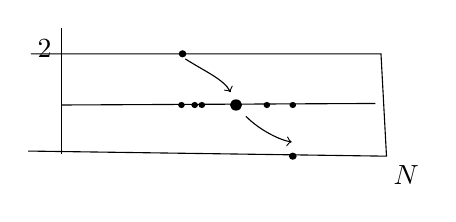
\begin{tikzpicture}[x=.7cm,y=.65cm]
\draw (0,.05)--(0,2.5);
\draw (-.55,2)--(5.8,2)--(5.9,0)--(-.6,.1);
\draw (0,1)--(5.7,1.03);
\node[left] at (0,2.1) {2};
\node[below right] at (5.85,0) {\(N\)};
\fill (2.2,2) circle (.07);
\foreach \x in {2.18,2.42,2.55,3.17,3.73,4.2}
{\fill (\x,1) circle (.06);}
\fill (3.17,1) circle (.11);
\fill (4.2,0) circle (.07);
\draw[->] (2.25,1.9)..controls (2.6,1.66) and (2.95,1.5)..(3.07,1.25);
\draw[->] (3.35,.78)..controls (3.6,.5) and (4,.3)..(4.18,.28);
\end{tikzpicture}}

avec \(E_2^{pq}=0\) si \(q\notin[0,2]\).
D'ailleurs \(R^0f_*(Q_l)\) est essentiellement \(Q_l\)
(du moins si \(f\) à fibres connexes, \unsure{ce que}
\unsure{l'on se ramène facilement}...],
donc les \deleted{\(R^pi_*\) sont} \(E_2^{p0}\) sont
\((d-1)\)-admissibles par \deleted{l'hyp.} ce qui vient d'être prouvé.

\deleted{Donc} D'autre part \(R^2f_*(Q_l)\simeq Q_l(-1)\), et
\[
E_2^{p2}\simeq R^pi_*(R^2f_*(Q_l))
\simeq\deleted{\unsure{E_2^{p2}}}
\inserted{Q_l(-1)}\deleted{\unsure{R^pi_*}}\otimes E_2^{p0}
\]
est donc également \((d-1)\) admissible, à fortiori
\deleted{\(\unsure{(d+d')}\)}
\inserted{\((d+d'-1)\)-}admissible
\inserted{i.e. \(d\)-admissible},
\deleted{Pour} On en conclut, utilisant lemme 2,
\inserted{et la constructibilité des \(E_2^{pq}\),}
que \(E_2^{p1}\) est une extension de \deleted{deux}\inserted{trois} faisceaux,
les extrêmes étant \deleted{\((d+d'-1)\)-\unsure{ad}} \(d\)-admissibles,
et le médian \unsure{des|est}
\[
E_3^{p1}=\cdots=E_\infty^{\unsure{p1|pq}}.
\]
Il suffit donc de prouver que \(E_\infty^{\unsure{p1|pq}}\) est \(d\)-admissible,
ou encore que \(R^n(if)_*(Q_l)\) l'est, ou encore que
\(R^n(gj)_*(\unsure{Q_l|Y})\) l'est,
ce qui par Leray et lemme 3 nous ramène au cas des
\(R^nj_*(Q_l)\), qui sont traités...
% archive foliation: 136
\scanpage{139}
\figure{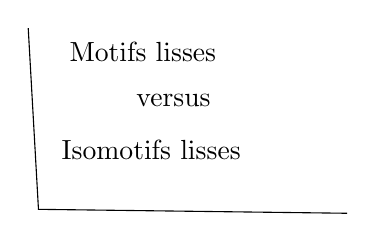
\begin{tikzpicture}[x=1cm,y=1cm]
\draw (0,2.3)--(.13,0)--(4.05,-.05);
\node[anchor=west] at (.4,2) {Motifs lisses};
\node[anchor=west] at (1.25,1.38) {versus};
\node[anchor=west] at (.3,.75) {Isomotifs lisses};
\end{tikzpicture}}
% archive foliation: 138
\scanpage{140}
\(S\) schéma normal intègre, pt générique \(\eta\), \(k(\eta)=K\).

\uline{Isomotif} (\(\frac12\) simple) \uline{lisse} sur \(S\) :
isomotif semi-simple \inserted{\(M\)} sur \(S\), tel que pour tout
\(l\in P\), \(l\ne\operatorname{car}K\), \(T_l(M)\) soit non ramifié rel. à
\(S_l=S[1/l]\).
Conjecturalement, il suffit que ce soit vrai pour \uline{un} \(l\)
premier à toutes les car. résiduelles
(\(\Longrightarrow\) il suffit que ce soit vrai pour \uline{deux} \(l\ne l'\)).

Motif (\unsure{isosemisimple|iso semisimple}) lisse sur \(S\)
(si \(\operatorname{car}K=0\)) :
\[
=\{M,\{E_l\},\{\alpha_l\}\}
\]
où

a) \(M\) un isomotif lisse sur \(S\)

b) \(\forall l\), \(E_l\) un faisceau \(l\)-adique \unsure{ct tordu|ctordu}
sur \(S_l=S[1/l]\) (ou donc sur \(K\), mais non ramifié rel. à \(S[1/l]\))

c) \(\forall l\), \(\alpha_l:E_l\otimes_{Z_l}Q_l\xrightarrow{\sim}T_l(M)\)

avec un axiome : ``pour presque tout \(l\), \(\unsure{u_l|\alpha_l}\)
provient d'un isomorphisme sur \(Z_l\) --- pas seulement à torsion près''.

Ceci implique que pour presque tout \(l\), \(E_l\) est sans torsion.

Homomorphisme de motifs lisses sur \(S\)
\[
(M,\{E_l\},\{\alpha_l\})\unsure{\mathbin{\text{---}}|\longrightarrow}(\unsure{M|M'},\{E'_l\},\{\alpha'_l\})
\]
\inserted{\(\unsure{u\to M}\)}
donné par \((u,\{u_l\})\), avec \(u:M\mathbin{\text{---}}M'\) un hom de
isomotifs, \unsure{à} et \(u_l:E_l\mathbin{\text{---}}\unsure{E_l|E'_l}\) un hom de
faisceaux \(l\)-adiques tels que pour \(\forall l\), on ait commutativité du
\diagram{\[
\begin{tikzcd}
E_l\otimes_{Z_l}Q_l\arrow[r,no head,"\alpha_l"]\arrow[d,no head,"u_l\otimes_{Z_l}Q_l"']&
T_l(M)\arrow[d,"\unsure{T_l(u)|T_l(M)}"]\\
E'_l\otimes_{Z_l}Q_l\arrow[r,no head,"\alpha'_l"']&T_l(M')
\end{tikzcd}
\]}

\uline{N.B.}\quad Le foncteur \deleted{\unsure{Hom}}
\[
\text{Motifs sur }K\longleftarrow\text{Motifs lisses sur }S
\]
est pleinement fidèle. Les Hom sont des modules de type fini sur \(Z\).
La catégorie des motifs lisses sur \(S\) est abélienne
(on prend \uline{noyaux}, conoyaux séparément pour les composantes \(M,E_l\)).
\deleted{Le foncteur} \inserted{L'image de}
\deleted{\unsure{Mot}}
(Motifs lisses sur \(S\)) dans (Motifs sur \(K\))
est une ss-catégorie abélienne \uline{épaisse}.

Le foncteur (Motifs\inserted{ lisses})
\(\longrightarrow\) (Isomotifs\inserted{ lisses}) est exact et surjectif
% archive foliation: 139
\scanpage{141}
% archive foliation: 140

La catégorie des groupes finis \inserted{comm. \(G\)} sur \(K\) tels que pour
\(\forall l\), \(G(l)\) soit non ramifié rel. à \(S[1/l]\), est une sous
catégorie épaisse de celle des motifs sur \(S\), la catégorie
quotient est équivalente à celle des isomotifs lisses sur \(S\).

La catégorie des motifs est une \(\otimes\)-catégorie avec
\uline{Hom}. Les foncteurs Motifs \(\longrightarrow\) isomotifs, motifs \(\longrightarrow\)
faisceaux \(l\)-adiques, sont des \(\otimes\)-foncteurs, compatibles aux
\uline{Hom}.

\unsure{Un|On} \deleted{définit} hom de motifs est une isogénie, s'il induit
un isom sur les isomotifs sous-jacents. On définit
la dimension (ou le poids), le niveau etc en termes
des isomotifs.

Tout schéma propre et lisse \(X\) sur \(S\) définit des
motifs \inserted{sur \(S\)} notés \(R^if_*(\mathbb Z_X)\), s'il n'y a pas de confusion à
craindre. De \(=\) pour les \unsure{sites} étales relatifs lisses et propres.

\uline{Relations avec les schémas en groupes commutatifs propres et lisses.}

On définit un foncteur \uline{contravariant} de la catégorie de
ces objets, soit \(A\), dans la catégorie des motifs sur \(S\),
en posant
\[
\deleted{\unsure{\varphi|\Phi}(A)=R^1f_*(\mathbb Z_A)=
(\quad R^1\unsure{f_*|f^*}(\quad}
\]
\[
\unsure{\varphi|\Phi}(A)=(M,E_l,u)
\]
où
\[
\left\{
\begin{aligned}
M&=R^1(f_{A^0})_*(\mathbb Q_{A^0})\\
E_l&=\underline{\operatorname{Hom}}({}_{l^\infty}A,\mathbb Q_l/\mathbb Z_l)\\
u_l&\ \text{provenant de l'hom évident}\\
&\qquad E_l\longrightarrow R^1f_{A^0*}(\mathbb Z_{lA^0})
\end{aligned}
\right.
\]
\margin{extension de \(\underline{\operatorname{Hom}}(A/A^0,\mathbb Q_l/\mathbb Z_l)\)
par \(R^1f_{A^0*}(\mathbb Z_{lA^0})\).}

\uline{NB} Il suffirait que \(A\)
\deleted{\(\unsure{/A^0|A^0}\) \illegible{2}}
\inserted{\unsure{soit} extension d'un schéma}
\unsure{gr. fini|en gr.} \(A/A^0\) par un schéma abélien \(A^0\), avec
\(A/A^0(l)\) extension par \(0\) d'un groupe fini étale sur \(S_{\unsure{l}}\).
\scanpage{142}
% archive foliation: 141

\uline{Le foncteur \(\unsure{\varphi|\Phi}\) est pleinement fidèle}
(On se ramène au cas de la base \(\eta=\operatorname{Spec}K\)).

L'image essentielle est \deleted{\uline{\unsure{évidemment|exactement}} \unsure{donc}}
formée des motifs \((M,\{E_l\},\{u_l\})\) tels que
\deleted{les \(E_l\)} leur quotient modulo
torsion est associé à un \uline{schéma} \uline{abélien} sur \(S\).
Il \uline{faut} pour cela que \(M\) soit effectif de poids \(1\),
i.e. est défini par un schéma abélien \inserted{\(A_K\)} sur \(K\).
\deleted{\(\unsure{A|R}\)} \deleted{\(M\)}.
La question si cette condition est suffisante revient à
celle-ci: Soit \(A\) un schéma abélien sur \(K\), \deleted{\unsure{de}} tel
que \(\forall l\), \deleted{les} \(T_l(A)\) soit non ramifié sur \(S_l\), alors
\(A\) a bonne réduction sur \(S\). Cela \unsure{marche} si
\(S\) est de dim \(1\), \inserted{(critère de \inserted{Néron-}Ogg-\unsure{Chafarevitch})},
\uline{ou} si de car. nulle (critère de
\unsure{critique|néronique}), mais peut-être pas au général [précisément
local régulier de dim \(2\) d'inégales caractéristiques]. Pour
faire un contre-exemple, il suffirait d'avoir un exemple
d'un schéma abélien \(A\) sur \(S\), et d'un sous-groupe fini de
\(A_K\) qui ne se prolonge pas en un sous-groupe fini et \uline{plat}
de \(A\). S'il y avait un tel exemple, il y en aurait
aussi avec un indice premier......

\margin{\uline{Pb} Avec la définition adoptée de motif lisse (en termes de
celle de isomotif lisse, comme un isomotif \uline{sur} \(K\)
avec simplement une propriété \inserted{``de lissité''} de non ramification pour
les \(T_l\)) il n'est pas du tout clair comment définir
l'image inverse d'un motif (resp. d'un isomotif) par
\(S'\mathbin{-}S\), p.ex. les fibres en les \(s\in S\). Cette difficulté
\deleted{se pose}\inserted{concerne}
--- tous les isomotifs, et vient déjà pour ceux qui sont effectifs de
poids \(1\).}
\scanpage{143}
% archive foliation: 142

Enveloppes pseudo-abéliennes
de catégories multiplicatives

(Construction abstraite de
Catégories de motifs).
\scanpage{144}
% archive foliation: 143

\uline{Construction abstraite d'une théorie de motifs semi-simples.}

On part d'une catégorie \(\mathcal V\)
\deleted{\unsure{pré}}``additive'', \deleted{\unsure{i.e.}}
\inserted{en particulier} les
\(\deleted{\operatorname{Hom}}\inserted{\operatorname{Fl}}(X,Y)\)
\deleted{\unsure{sont}} munis de une structure de
groupe abélien, les accouplements de composition
étant bilinéaires.
\deleted{[On ne suppose pas qu'il
existe un objet nul, et des sommes \unsure{pour deux}
\unsure{ou deux|de deux} objets......]}.
On s'intéresse, pour
toute catégorie \uline{abélienne} \(\mathcal C\), aux foncteurs
\deleted{contravariants} ``additifs''
(i.e. commutant aux sommes
finies, --- \inserted{\unsure{ce|ou} qui revient au \(=\)} aux pr. directs finis)
\[
H\deleted{\unsure{\,\mathcal V}}:
\mathcal V^{\unsure{\circ|*}}\longrightarrow\mathcal C
\]
et on cherche un foncteur universel
de cette nature
\[
\underline h:\mathcal V^{\unsure{\circ|*}}\longrightarrow\mathcal M(\mathcal V)=\mathcal M
\]
foncteur additif dans catégorie abélienne \(\mathcal M\)) tel
que pour toute catégorie abélienne \(\mathcal C\),
l'application
\[
\begin{gathered}
T\longmapsto T\circ\underline h\\
\operatorname{Fonc\,exacts}(\mathcal M,\mathcal C)
\longrightarrow\operatorname{Fonc\,add}(\mathcal V^{\unsure{\circ|*}},\mathcal C)
\end{gathered}
\]
soit bijective (ce qui caractérise \(\mathcal M\) à \deleted{isomorphisme}
isom près), ou le cas échéant, que
\[
\underline{\operatorname{Fonc\,exacts}}(\mathcal M,\mathcal C)
\mathbin{-}
\underline{\operatorname{Fonc\,add}}(\mathcal V^{\unsure{\circ|*}},\mathcal C)
\]
soit une équivalence de catégories, \unsure{ce qui|c à qui}
\scanpage{145}
% archive foliation: 144

caractérise \(\mathcal M\) à équivalence près). De plus, on
\unsure{aime|vise} donner des conditions moyennant
lesquelles le foncteur \(\underline h\) est \uline{pleinement}
\uline{fidèle}.

On va supposer que la structure \deleted{pré}additive
sur \(\mathcal V\) peut s'enrichir en une structure
\(\unsure{k|Q}\)-linéaire, où \(Q\) est un \uline{corps} commutatif,
[NB. si \(Q=\mathbb Q\), est évidemment déterminée
de façon unique]. On suppose que les
\deleted{\(\unsure{\operatorname{Hom}}\)}
\deleted{\(\operatorname{Fl}(X,Y)\) sont des vectoriels de dim
finie sur \(k\), et} que pour \(\forall X\), \(\operatorname{Fl}(X,X)\) est
une \uline{algèbre} \inserted{\uline{de dim finie}}
\uline{semi-simple} sur \(\deleted{k}\). Nous allons
alors \deleted{\unsure{en}} construire une catégorie \(\mathcal M^{\unsure{\sharp|*|\natural}}\) de la
façon suivante. Un objet de \(\mathcal M^{\unsure{\sharp|*|\natural}}\) est
un couple \((X,\pi)\), où \(X\in\operatorname{Ob}\mathcal V\), \(\pi\in\operatorname{Fl}(X,X)\),
\(\pi^2=\pi\) (\(\pi\) est un \uline{projecteur} de \(X\)). Un
homomorphisme \((X,\pi)\longrightarrow(X',\pi')\) est
un hom \(f:X\longrightarrow X'\) tel que
\(\pi'f=f\pi\), \uline{modulo} les \(f\) tels que
\(f\pi=\pi'f=0\). On compose de façon
évidente. D'où une catégorie, \inserted{\(\mathcal M^{\unsure{\sharp|*|\natural}}\)}, manifestement additive,
et un foncteur additif

\margin{i.e. \unsure{on a un hom} d'anneaux
\(Q\mathbin{-}\operatorname{End}\operatorname{id}_{\mathcal V}\)}

\diagram{
\begin{tikzcd}[column sep=large,row sep=large]
X \arrow[r,no head,"\pi"] \arrow[d,"f"'] &
X \arrow[d,no head,"f"]\\
X' \arrow[r,no head,"\pi'"] \arrow[d,no head,"g"'] &
X' \arrow[d,no head,"g"]\\
X'' \arrow[r,no head,"\pi''"] & X''
\end{tikzcd}
}
\scanpage{146}
% archive foliation: 145

évident, d'ailleurs pleinement fidèle
\[
\underline h^{\unsure{\sharp|*|\natural}}:\mathcal V\longrightarrow\mathcal M^{\unsure{\sharp|*|\natural}}
\]
en posant \(\underline h^{\unsure{\sharp|*|\natural}}(X)=(X,\operatorname{id}_X)\).
Pour toute catégorie
abélienne \(\mathcal C\), le foncteur \(\varphi:T\longmapsto T\circ h\)
\[
\underline{\operatorname{Fonc\,add}}(\mathcal M,\mathcal C)
\xrightarrow{\varphi}
\underline{\operatorname{Fonc\,add}}(\mathcal V,\mathcal C)
\]
est une \deleted{isomorphisme} équivalence. Pour le voir, on
se construit un foncteur quasi-inverse
\deleted{(1) pleinement fidèle. Un}
\[
\psi:\underline{\operatorname{Fonc\,add}}(\mathcal V,\mathcal C)
\longrightarrow
\underline{\operatorname{Fonc\,add}}(\mathcal M,\mathcal C)
\]
en associant à \unsure{un} foncteur \inserted{additif}
\(H:\mathcal V\mathbin{-}\mathcal C\)
son extension canonique
\[
\psi(H)(X,\pi)=\operatorname{Im}H(\pi)
\]
avec la loi fonctorielle évidente. On voit
aussitôt que l'on a des isom can
\[
\begin{aligned}
\varphi(\psi\unsure{)}(H)&\simeq H\\
\psi\varphi(T)&\simeq T
\end{aligned}
\]
Pour l'instant, cette construction et propriété
universelle de \(\mathcal M\) n'utilise pas les hyp
précédentes faites sur \(\mathcal V\); elle répond au Pb
universel de \uline{rendre tous les projecteurs
scindables} \inserted{(d'une catégorie additive donnée)}.
Mais les hypothèses faites
sur \(\mathcal V\) vont impliquer que \(\mathcal M\) est en
fait une catégorie \inserted{\uline{abélienne}} \uline{semi-simple}
(i.e. tout objet de

\margin{il suffit que \(\mathcal C\) soit une catégorie additive où
les projecteurs sont scindables}
\scanpage{147}
% archive foliation: 146

\unsure{permet de se ramener}: un objet
\(P\) de la forme \(\underline h(X)\),
\deleted{\unsure{donc} \(u\) de la forme
\(\underline h(\alpha)\), où \(\alpha\in\operatorname{Fl}(X,X)\). Or comme}
\inserted{\(\operatorname{Fl}(P,P)\simeq\operatorname{Fl}(X,X)\), donc}
\(\operatorname{Fl}(P,P)\) est un \uline{anneau semi-simple} \(U\), \deleted{\unsure{Q}}
\deleted{Pour un tel anneau, tout \unsure{idéal opérant}
sur un objet d'une catégorie}
\inserted{Alors \(P\) et \(u\) se décomposent suivant les
composantes simples de \(U=\operatorname{Fl}(P,P)\) (i.e. de son
centre)}
\deleted{et on est ramené au cas où \(U\)}

Or lorsque un anneau de ce type opère
sur un objet d'une catégorie abélienne, alors
pour tout \(u\in U\), on peut trouver
\deleted{deux couples
d'idempotents orthogonaux complémentaires \(\pi,\pi'\) de \(U\),
\unsure{tels que}
\((\pi\pi'=\pi'\pi=0,\quad\pi+\pi'=1,\quad\pi^2=\pi,\quad\pi'^2=\pi')\)
tels que
et \(\varpi,\varpi'\) tels que}
\(u\pi'=0,\ \varpi'u=0,\)
\inserted{\(v\in U\) tel que
\(vu\) soit un \deleted{projecteur}\inserted{idempotent} \(\pi\)
\(uv\) soit \(\mathbin{-}\ \varpi\)}

\diagram{
\begin{tikzcd}[column sep=large,row sep=large]
P\simeq\pi P+\pi'P \arrow[r] & \pi P \arrow[d,"\unsure{\sim}"]\\
Q\simeq\varpi Q+\varpi'Q & \varpi Q \arrow[l]
\end{tikzcd}
}

\diagram{
\begin{tikzcd}[column sep=large,row sep=large]
P \arrow[r,"u"] \arrow[d] &
\unsure{Q} \arrow[l,bend right=40,"v"']\\
P' \arrow[r,"\simeq"] & Q' \arrow[u]
\end{tikzcd}
}

\[
\left\{
\begin{aligned}
vu&=\text{projecteur }\pi\\
uv&=\text{projecteur }\varpi\\
&\deleted{\unsure{vu}}
\end{aligned}
\right.
\]
\inserted{\figure{\begin{tikzpicture}[x=1cm,y=1cm]
\node at (0,0) {\(\begin{gathered}
\pi v=v,\quad u\pi=u\\
\varpi u=u,\quad v\varpi=v
\end{gathered}\)};
\draw (0,0) ellipse (2.25cm and .7cm);
\node[anchor=west] at (1.7,2.05) {et on a les relations};
\draw[->] (1.8,.5)..controls (2.5,1.3) and (4.9,.55)..(5.1,1.85);
\end{tikzpicture}}}
de cette façon,
gagne donc.

Pour les conditions de chaînes, on
utilise le fait que les \(\operatorname{Fl}(X,X)\) sont
de \deleted{\unsure{degr}} dim finie sur \(k\). .....

\diagram{
\begin{tikzcd}[column sep=large,row sep=large]
P'+P'' \arrow[d,shift left,"\unsure{\pi|\simeq}"'] & Q'+Q'' \arrow[d,shift left]\\
P' \arrow[u,shift left] \arrow[r,shift right] &
\unsure{Q'|Q} \arrow[u,shift left] \arrow[l,shift right]
\end{tikzcd}
}
\scanpage{148}
% archive foliation: 147

cette catégorie est semi-simple). Si donc \(\mathcal C\) est
une catégorie abélienne, les foncteurs additifs
de \(\mathcal M\) dans \(\mathcal C\) sont autom. exacts. Cela
prouve que le ``Pb universel'' \inserted{(avec un grain de sel)}
en termes
de catégories abéliennes (Variante \(2\)) est
résolu par \(\mathcal M\).

Prouvons donc que \(\mathcal M\) est une catégorie
\uline{abélienne} \uline{semi-simple}. Cela équivaut à ceci:

\deleted{tout morphisme est \unsure{dir}}
\unsure{(i)|(iv)} Tout objet \deleted{\(\unsure{X}\)} satisfait condition des chaînes ascendantes,
et descendantes pour les \unsure{ss-objets|sous-objets} facteurs directs,

\deleted{i.e. \unsure{l'on a|l'est} des \unsure{pr}}
(ii) Tout morphisme \(u:P\longrightarrow Q\) est ``direct'',
i.e. isom à un morphisme
\[
A\times B\xrightarrow[\operatorname{inj}_1\circ\operatorname{pr}_2]{}B\times C
\]

Pour vérifier (ii), \deleted{\unsure{considérons}} considérons \(R=P\times Q\),
et l'endomorphisme \(\deleted{\unsure{pr}}\ v=\operatorname{inj}_2u\operatorname{pr}_2\) de \(R\).
On voit aisément que pour \deleted{\unsure{que}} (ii) \inserted{soit vrai}
pour \(u\),
il \inserted{\(^{(*)}\)} suffit \deleted{de} qu'il le soit pour \(v\), donc on
est ramené au cas où \(P=Q\). D'autre part,
soit \deleted{\(\unsure{R}\)} \(S\) un autre objet, et sur
\(R=P+S\), \(v=u\oplus0_S\), alors on constate que la
propriété est vraie pour \(u\) ssi elle l'est pour \(v\). Cela nous

\margin{\((*)\) dans un \unsure{carré} commut.
il est innocent de modifier
\(P\longrightarrow Q\) par
\(P\unsure{\in|\subset}P',\ Q\unsure{\in|\subset}Q'\)
\diagram{
\begin{tikzcd}[column sep=small,row sep=small]
&&Q'\\
{} \arrow[r] & P \arrow[r] & Q \arrow[u]
\end{tikzcd}
}}
\scanpage{149}
% archive foliation: 148

On suppose donné trois catégories \inserted{additives}
\(\mathcal V,\mathcal V',\mathcal V''\),
d'où \(\mathcal M,\mathcal M',\mathcal M''\); on suppose donné un
foncteur bi-additif \(\mathcal V\times\mathcal V'\mathbin{-}\mathcal V''\).
Alors il se
prolonge de façon \(\unsure{\mathrm{ess}^{t}}\) unique en un
foncteur bi-additif \(\mathcal M\times\mathcal M'\mathbin{-}\mathcal M''\).
En fait,
on voit que la propriété \inserted{\unsure{pseudo}-}universelle qui
définit \(\mathcal M\) en termes de \(\mathcal V\), s'étend aux
bifoncteurs, .....

On \deleted{\unsure{l'}} utilisera cette construction surtout
pour un bifoncteur \(\mathcal V\times\mathcal V\mathbin{-}\mathcal V\)
``\uline{symétrique}'', et ``\uline{associatif}''
\inserted{et ``unitaire''}, noté \(\deleted{\otimes}\ \boxtimes\).
Alors
on trouve un bifoncteur de \(=\) nature dans
\(\mathcal M\), noté \(\otimes\). Si \(k\) est \uline{de car. \(0\)}
\inserted{(p.ex. \(\unsure{\mathbb Q|Q}\))}, on peut
construire alors toutes les opérations tensorielles \inserted{\uline{covariantes}}
dans \(\mathcal M\) [en plusieurs arguments], par
exemple on pourra définir les
\[
\overset{\unsure{n}}{\otimes}M,\quad
\overset{n}{\wedge}M,\quad
\deleted{\text{et}} S^n(M)\quad\text{etc}\ \ldots.
\]
